%%%%%%%%%%%%%%%%%%%%%%%%%%%%%%%%%%%%%%%%%%%%%%%%%%%%%%%%%%%%%%%%%%%%%%%%%%%%%%%%
%2345678901234567890123456789012345678901234567890123456789012345678901234567890
%        1         2         3         4         5         6         7         8
%\documentclass[smallextended,natbib]{svjour3}
\documentclass[twocolumn]{svjour3}       % twocolumn (second format)
%\documentclass[smallextended]{svjour3}       % onecolumn (second format)

%
\smartqed  % flush right qed marks, e.g. at end of proof
%
\usepackage[numbers]{natbib}
\usepackage{makeidx}         % allows index generation
\usepackage{graphicx}        % standard LaTeX graphics tool
\usepackage{multicol}        % used for the two-column index
\usepackage[bottom]{footmisc}% places footnotes at page bottom
\usepackage{graphics}
\usepackage{times} % assumes new font selection scheme installed
\usepackage[fleqn]{amsmath} % assumes amsmath package installed
\usepackage{amssymb}  % assumes amsmath package installed
\usepackage{mathrsfs}
\usepackage{subfigure}
\usepackage{enumerate}
\usepackage{csquotes}
\usepackage{marvosym} 
\usepackage{array}
\usepackage{kpfonts}
\usepackage{amsmath} % assumes amsmath package installed
\usepackage{mathrsfs}
\usepackage{color}
\usepackage{comment}
\usepackage{hyperref}
\hypersetup{
     colorlinks   = true,
     citecolor    = blue,
		linkcolor=blue
}
\usepackage{multirow}
\usepackage{float}
\usepackage{enumerate}
\usepackage{algorithm}
\usepackage{algorithmic}

\newtheorem{mytheorem}{Theorem}
\newtheorem{myremark}{Remark}
\newtheorem{mylemma}{Lemma}
\newtheorem{mydef}{Definition}
\newtheorem{myprob}{Problem}

%
\journalname{Journal of Intelligent and Robotic systems}
%
%%%%%%%%%%%%%%%%%%%%%%%%%%%%%%%%%%%%%%%%%%%%%%%%%%%%%%%%%%%%%%%%
\begin{document}

\title{Multi-robot deployment on topological maps}


%\titlerunning{Short form of title}        % if too long for running head

\author{Reza J. Alitappeh \and Guilherme A. S. Pereira \and Arthur R. Ara\'ujo \and Luciano C. A. Pimenta  }

%\authorrunning{Short form of author list} % if too long for running head

\institute{R. Alitappeh (\Letter) \and G. Pereira  \and A. Ara\'ujo \and L. Pimenta\at School of Engineering,           Universidade Federal de Minas Gerais~(UFMG), Belo Horizonte, MG 31270-901, Brazil \\
Tel.: +55 (31)3409-5465\\
Fax: +55 (31)3409-5480\\
R. Alitappeh \\
\email{rezajavanmard@ufmg.br} \\
G. Pereira \\
\email{gpereira@ufmg.br} \\
A. Ara\'ujo \\
\email{araujoarthur0@hotmail.com} \\
L. Pimenta \\
\email{lucpim@cpdee.ufmg.br}
}

\date{Received: date / Accepted: date}
% The correct dates will be entered by the editor


\maketitle

\begin{abstract}

This paper proposes an efficient deployment strategy to optimally distribute teams of robots in environments that can be represented by topological maps. Among the several applications for our solution are sensing and coverage of large corridor-based buildings, such as hospitals and schools, and the optimal placement of service vehicles in the streets of a big city. The representation of the environment as a topological map transforms the original two or three-dimensional problem into a one-dimensional, simplified problem, thus reducing the computational cost of the solution. Moreover, after the computation of the optimal solution, each robot can reach its final position by simply following a sequence of intuitive, human-like commands, without the need for global metric localization, which also simplifies robot control. %{\color{blue} Does this mean that our method is centralized? Guilherme: Lets not mention that. It does not matter!}
Besides presenting convergence proofs for our method, the paper also presents simulated and real world experiments that illustrate and validate our approach.
\keywords{Multi-robot deployment \and Topological map \and Multi-robot coverage \and }

\end{abstract}

%%%%%%%%%%%%%%%%%%%%%%%%%%%%%%%%%%%%%%%%%%%%%%%%%%%%%%%%%%%%%%%%%%%%%%%%%%%%%%%%
\section{Introduction}

Among the different research topics in the area of cooperative and distributed robotic systems, the \textit{multi-robot deployment problem} appears as one of the more studied ones~\cite{DistCtrlRobotNetw}. In fact, distributing a team of mobile robots in a known workspace is one of the fundamental tasks in multi-robot systems. Applications for robot deployment include sensing and coverage, where the robots are distributed in an environment and respond to the events that occur in their dedicated region. 

The first distributed technique for multi-robot deployment was proposed  by Cortes et al.~\cite{Cortes2004} based on Lloyd's framework~\cite{Lloyd1982}. In that work, robots were deployed over a convex environment based on a continuous control law that minimized a functional representing the quality of the deployment. 
%
A density function represented the priority of points inside a region, so that higher priority points must be better covered. Coverage in the sense of~\cite{Cortes2004} is illustrated in Fig.~\ref{fig:sampledeplyoment}. In this figure four robots are deployed in a convex environment. The density function used is uniform, so all points of the environment have identical priority. At the beginning, the environment is divided in four Voronoi regions\footnote{A Voronoi region for a robot is composed by all points closer to that robot than to any other robot.}, one for each robot. The technique proposed in~\cite{Cortes2004} generates velocity vectors for each robot so that they continuously move towards the centroids of their respective Voronoi regions, which, as a consequence, change the region itself, as show in Fig.~\ref{fig:sampledeplyoment}. As the time evolves, it can be proved that the multi-robot system converges to a configuration where the environment is equally distributed among the robots or, in the case of non-uniform density functions, is distributed according to this function. It is important to notice that, even in convex workspaces, real world implementations of this methodology require global and precise metric localization for the robots and non-linear control strategies to follow the velocity vectors. 

\begin{figure}[b]
\centering
\subfigure[Time 1.]{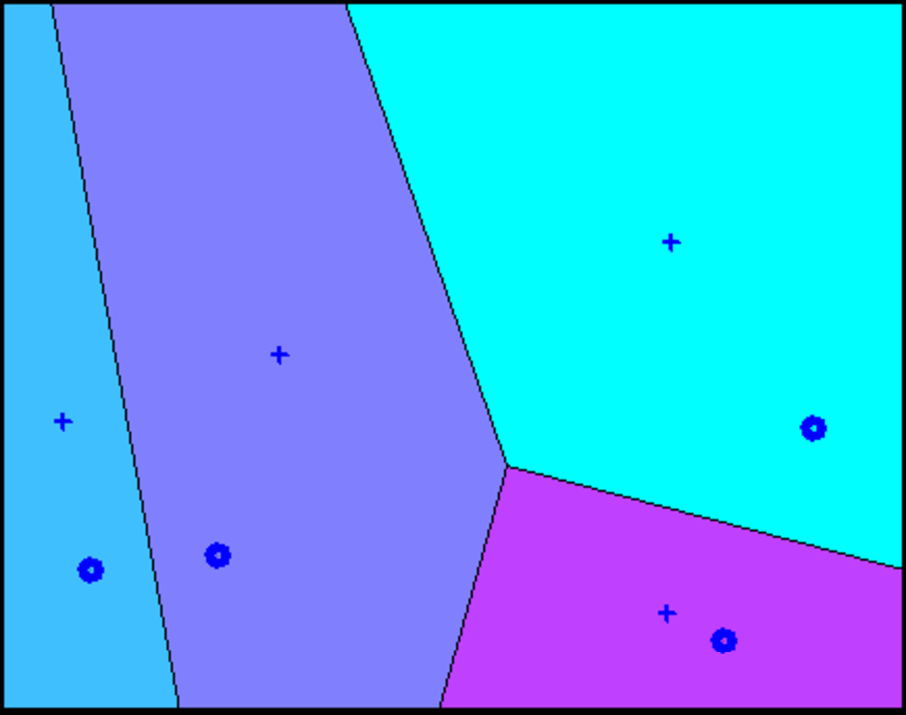
\includegraphics[width=0.3\columnwidth]{Figures/Iter1.pdf}} 
\subfigure[Time 4.]{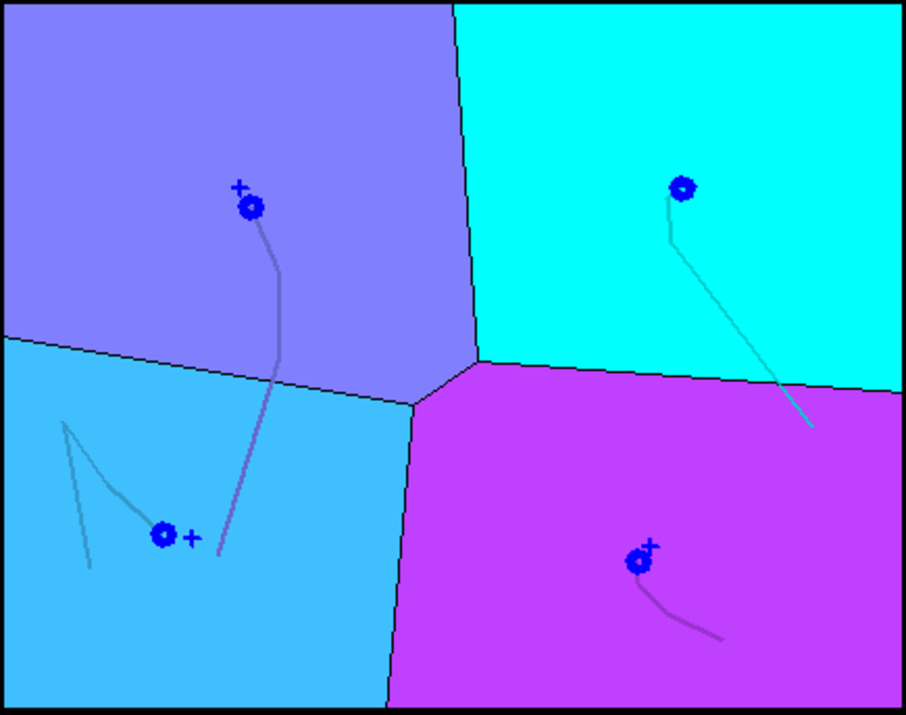
\includegraphics[width=0.3\columnwidth]{Figures/Iter4.pdf}}    
\subfigure[Final.]{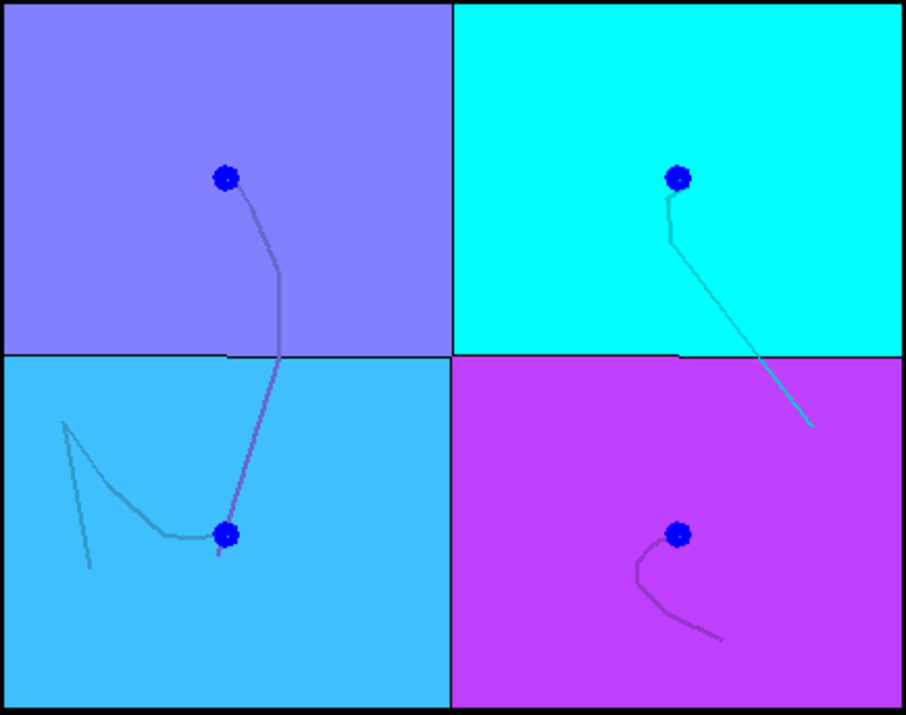
\includegraphics[width=0.3\columnwidth]{Figures/Iter12.pdf}}    
\caption{Deployment of 4 robots in a convex environment using the approach proposed by~\cite{Cortes2004}. In (a) and (b) the ``+" sign indicates to the center of the Voronoi regions, which represent the current goal position for each robot. Voronoi regions are highlighted with different colors.}
\label{fig:sampledeplyoment}
\end{figure}

Different extensions for this strategy were developed by several authors. This extensions can be classified by different aspects.
As shown in Table~\ref{tbl:classification}, the several previous solutions encountered in the literature can work in convex or non-convex environment, be distributed or centralized, use Euclidean, geodesic or geodesic GVD distance metrics, generate continuous or discrete control actions, and finally, be based on geometric or grid maps. 

The main contribution of the methodology presented in this paper is the use of graph based topological maps to model the robot's workspace. Independently of the dimension of the original workspace, this strategy transforms the problem into a one dimensional problem, what highly increases the computational efficiency of the method, thus allowing for the deployment of large teams of robots in very extensive workspaces. Due to the use of a topological map, in our approach the robots may be controlled using a sequence of human like commands, such as ``turn right'', ``turn left'' and ``move straight''. Also, no global metric localization is required. Our approach  was designed to be applied in structured, usually non-convex workspaces, that are suitable for topological mapping. These include metropolitan regions composed by streets and intersections, pi\-pe\-lines and energy distribution systems with several connections and bifurcations, and large buildings with intersecting corridors. Since in many applications of real world robots can not be controlled by a centralized system, our method is fully distributed  in a way each robot needs to communicate only with its neighbors. Also, the proposed strategy is provable correct in the sense that robot positions converge to the optimal locations in the topological map. As a drawback, it is important to mention that, these topological locations do not necessarily correspond to optimal positions in the real workspace, which makes the quality of the deployment dependent on the map discretization. 

Before we present our methodology, next section will present a brief review of the multi-robot deployment area. The rest of the paper is divided at it follows: problem statement is in Section~\ref{sec:probstate}; Section~\ref{sec:methodology} is dedicated to present the proposed methodology, including the discretization technique, the topological map model, the methodology itself and the convergence proofs; Simulations and actual robot experiments are in Section~\ref{sec:implementation}; Finally, in Section~\ref{sec:conclusion} we conclude the paper and present some ideas for future research.

\section{Literature Review}

%As it is shown in Table~\ref{tbl:classification}, state of the art are applicable 

\begin{table}[t]
\centering
\caption{Different classes of deployment approach (abbreviation are used for convex "Conv." (non-convex, "n-Conv. "),Euclidean, "Eucl.", geodesic, "Geo.", discrete, "Des." continuous "Cont." and heterogeneous, "Hetr." )   }
\label{tbl:classification}
\begin{tabular}{m{1.8cm}m{1.2cm}m{0.8cm}m{0.55cm}m{0.55cm}c}
Methodology                  	      & environment   & metric     & setup 	& Hetr. & map    \\
 \hline
 \\
 2004, \cite{Cortes2004}      		 & Conv.     	      &  Eucl. & Con.  		&	 ~~- & geometric	\\
 2008, \cite{Pimenta2008},\cite{Pimenta2088SCAT}&n-Conv.&  Geo.  & Con.  		& Hetr.& geometric \\
 2009, \cite{Schwager2009}    		 & Conv.    		  &  Eucl. & Con.		&  ~~- & geometric   \\
 2010, \cite{Breitenmoser2010} 		 & n-Conv.	      &  Geo.  & Con.   	&  ~~- & geometric	\\
 2011, \cite{Stergi2011}    	     & Conv.  	 		  &  Eucl. & Con. 	 	& Hetr.& geometric \\
 2011, \cite{Schwager2011}	   		 & n-Conv. 		  &  Eucl. & Con. 	 	& ~~-    & geometric \\
 2012, \cite{Mahboubi2012}     		 & Conv. 		  &  Eucl. & Con. 		&  ~~-   & geometric \\
 2012, \cite{Durham2012}	  		 & n-Conv. 	      &  Geo.  & Des. 		& Hetr.*& grid\\
 2013, \cite{Yun2013}        		 & n-Conv.		  &  Geo.  & Des. 		&   ~~-  	& grid \\
 2013, \cite{Bhattacharya2013IJRR},\cite{Bhattacharya2013a}		 & n-Conv. 	      &  Geo.  & Con.*    	&  ~~- 	& geometric\\
 2014, \cite{reza2014} 		  		 & n-Conv. 		  & Geo. GVD& Con.*      &  ~~- 	& grid\\
 2014, \cite{Sharifi2014}  	  		 & Conv. 	  	     & Eucl.   & Con.       &  ~~- 	& geometric\\
 2015, \cite{Sharifi2015},\cite{Pierson2015}  	  		 & Conv. 	  	     & Eucl.   & Con.       &  Hetr. & geometric\\
%  2015, \cite{Pierson2015}  	  		 & Conv. 	  	     & Eucl.   & Con.       &  Hetr. & geometric\\
\textbf{This paper}				  		 &\textbf{n-Conv.}	     &\textbf{Geo.}& \textbf{Dec.}       &  \textbf{Hetr.} & \textbf{topologic}\\
 \hline
 \\
 \multicolumn{6}{m{8cm}}{ Con.* : A continues setup with discrete approximation}\\
 \multicolumn{6}{m{8cm}}{ Hetr.* : The method has the potential to work in Heterogeneous model.}
\end{tabular}
\end{table}
%

This section will survey the main works in the area of multi-robot deployment. For a chronological order and characteristic of each method presented, please refer to Table~\ref{tbl:classification}. 

After the initial  work~\cite{Cortes2004}, which can only be applied to convex and static environments, Pimenta et al.~\cite{Pimenta2008}, applied geodesic distance for deploying a team of heterogeneous robots in non-convex environments. Time-varying density function was addressed in~\cite{Pimenta2088SCAT}. For a similar problem, in~\cite{Schwager2009}, an adaptive controller is developed, where robots learn the distribution of sensory information (density function) during the deployment.
Another approach for deploying multiple robot in non-convex environment was presented in~\cite{Breitenmoser2010}. In order to avoid collision with obstacles, the authors combined the deployment control law with a local planner (Tangent Bug).

Most of the previously cited works can be classified as Voronoi-based coverage strategies since they use the centroid of the current Voronoi region in their controller. However, there are other papers that provide alternative partitioning techniques. In~\cite{Tzes2010}, authors proposed a space-partitioning for heterogeneous network, which had less computation compared to the existing techniques. In another work~\cite{Stergi2011}, a distributed controller was derived for a heterogeneous mobile sensor network with different sensing radii based on the modified Voronoi defined in~\cite{Tzes2010}.
%
Another different partitioning scheme was proposed by Mahboubi et al. in~\cite{Mahboubi2012}, where Multiplicative Weighted (MW) Voronoi  diagram and Visibility-aware Multiplicative Weighted (VMW) Voronoi diagram were used in environments with and without obstacles, respectively. In their work, the authors defined different weights for each robot during the construction of the Voronoi tessellation.
%
A deployment strategy for multi-agent system that considered communication delay and sensors effectiveness variation is presented in~\cite{Sharifi2014}. In this work a new partitioning technique is developed in order to address variation in sensors behavior, which is called Guaranteed Multiplicative Weighted (GMW) Voronoi.
%
Agents with different types of dynamics are taken into account by the same authors in~\cite{Sharifi2015}. They used MV-Voronoi partitioning approach to find corresponding region for each robot based on their dynamic.
% They applied the same idea to in. The problem is investigated for the case where agents have different types of dynamics. Using a multiplicatively-weighted Voronoi diagram, the field is partitioned to smaller regions (one for each agent).

%---------------------------- compare to our method
While the approaches cited above focused on environments with two or three dimensions represented by geometric maps, in this paper a discrete, one-dimensional topological map is used to represent the robot's workspace. As it usual, the topological map is represented by a graph, in our case a direct graph.
% 
There are some previous studies in discrete space deployment. For instance, in~\cite{Durham2012} the authors represent the environment using grid cells and a discrete coverage optimization algorithm is applied on robots with short-range communication.
% 
In~\cite{Bhattacharya2013a} and~\cite{Bhattacharya2013IJRR} Bhattacharya et al. tried to approximate the continuous control setup with a discrete version. They discretized a non-convex environment and represented it as a graph. Standard graph search algorithm was employed in order to compute the control law.
%
Safe deployment problem was considered by Javanmard  and Pimenta in~\cite{reza2014}, where a new metric based on Generalized Voronoi Diagram (GVD) (called Geodesic GVD) yields a safe motion for a team of robots. In their implementation, a discrete approximation with graph representation is also used. 

Among all previous approaches surveyed, the most similar to the one present in this paper is~\cite{Yun2013}. The authors computed the Voronoi partitions upon an undirected graph that topologically encodes the environment. However, the authors still use the original 2D metric map to control the robots, what, similarly to all other previous strategies, makes the method dependent on precise distance and localization. The approach proposed in the present paper improves on that point once all steps of the method execute on the topological map. This highly simplifies the the actual robot implementation, as will be clear in the rest of the text.

%
The main idea behind our methodology was inspired by~\cite{Arthur2015}, where a robot uses human-like commands to move in a structured environments. In fact, humans do not need to have a precise metric localization to reach a destination. A simple sequence of directions such as "turn right", "turn left", and "go straight" may be enough for a person to reach its destination in a urban environments or office building. Our methodology uses graph search strategies to generate such sequences of commands and deploy the robot team in the environment. 
%
This can be considered as a milestone in the literature of deployment, since it does not require a specific metric for the computation. As for the humans, metric localization is also not necessary. Given a robot that is able to move without the need of localization (by following walls or driveways, for example), high speed motion and fast response can be achievable. Arguably, this method is suitable for emergency responses like chasing an evader or responding to accidents etc. It is important to remark that the proposed technique also does not need a complete and precise map as input, since it can even be applied on partially known or even manually sketched maps. %Thus our approach can conduct robots to be deployed in an environment, where the map is not completely available or when for example a disaster destroyed a part of the map. 
In the next section we precisely define the problem considered in this paper.  

%
%%%%%%%%%%%%%%%%%%%%%%%%%%%%%%%%%%%%%%%%%%%%%%%%%%%%%%%%%%%%%%%%%%%%%%%%%%%%%%%%
%%%%%%%%%%%%%%%%%%%%%%%%%%%%%%%%%%%%%%%%%%%%%%%%%%%%%%%%%%%%%%%%%%%%%%%%%%%%%%%%
\section{Problem statement}
\label{sec:probstate}

In a discrete environment, let $G(\mathcal V,\mathcal E)$ be a complete graph representing a map  $E \subset \mathbb{R}^2$, where $\mathcal V$ and $\mathcal E$ are set of vertices and edges in $G$. 
%
A team of $n$ robots are distributed randomly in the environment to cover the field, so that the configuration of the $i^{th}$ robot is presented by $r_i \in \mathcal V$, and $R=\{r_1,\cdots,r_n \}$. Furthermore, a density function $\phi: \mathcal{V} \rightarrow \mathbb{R}^+$ indicates the importance of the vertices in $G$, in which vertices with large values of $\phi$ have more priority in being covered. 
%
%##################################################
\begin{myprob}[Discrete locational deployment problem]
\label{Prob:deployment}
\qquad \qquad \qquad
%
\textnormal{
By considering above explanation, we can define the discrete deployment function $\mathcal{H}$ (similar to what is defined in \cite{Yun2013}) as follows:}
%
\begin{equation}\label{eq:functional1}
\mathcal{H}(R,W) =
\sum_{i = 1}^{n} \sum_{q \in w_i}
d(q, r_i)\phi(q) \,,
\end{equation}
%
\textnormal{
where $d(q,r_i)$ is a function $d:\mathcal V \times \mathcal V \rightarrow \mathbb R^+$ denotes the shortest path between a vertex $q$ and robot $i$. And the set $W=\{w_1,\cdots,w_n\}$ states $n$ partitions of $G$.}
\end{myprob}

An intuitive perception of $\mathcal{H}$ indicates the quality of deployment, for example in figure \ref{fig:sampledeplyoment} (c) we obtained the optimum value of this function which means robots deployed at the center of dedicated partitions, whereas partitions are equally divided between robots.
%
In this discrete formulation (\ref{eq:functional1}), the main objective is minimizing $\mathcal{H}$ function, so that robots will be located on vertices in their corresponding partitions, $W$, where they have minimum distance to the assigned region. Later every robot is responsible about events happening in vertices within.

In such a distributed strategy each robot computes its deployment function $\mathcal{H}_i$ (\ref{eq:functional2}) individually. 
%
\begin{equation}
\label{eq:functional2}
\mathcal{H}_{i}(r_i,w_i) = \sum_{q \in w_i}
d(q, r_i)\phi(q) \,,
\end{equation}

In this way, robots need to establish a connection with the neighbor robots to receive their locational information. We show a set of neighbors $\mathcal{N}_i$ by $\mathcal N_i=\{j~|~w_i \cap w_j \neq \emptyset, i \neq j \}$, which means robot $j$ is a neighbor of robot $i$ if they have a common boundary. It is assumed that the information of the environment $G$ and density function $\phi$ are available for all robots initially. 

In this discrete setup for controlling the robots toward minimizing the deployment function $\mathcal{H}$ different strategies were applied, i. e. in \cite{Durham2012} and \cite{Yun2013} authors proposed a discrete controller inspired from the continuous control law proposed by Cortes in \cite{Cortes2004}. Such that every robot moves to the center of region $w_i$, iteratively. In another word, for the robot $i$, the algorithm searches among the nodes in its corresponding region $w_i$, in order to find the node minimizes the $\mathcal{H}_i$ in the current iteration. In both methods their computation depends on the size of the current region for every robots, since they recompute Eq. (\ref{eq:functional1}) for the entire number of vertices of the graph in each iteration.

In section \ref{sec:methodology} we explain how we modify this setup to be applicable in topological map space with drastically lower complexity and also provable in the sense of convergence.

%%%%%%%%%%%%%%%%%%%%%%%%%%%%%%%%%%%%%%%%%%%%%%%%%%%%%%%%%%%%%%%%%%%%%%%%%%%%%%%%

\section{Methodology}
\label{sec:methodology}


In this section we explain a new graph representation of the topological map and the distributed deployment algorithm. Moreover, the proof of convergence is discussed at the end of this section.

%######################################
\subsection{Topological map representation}
\label{sec:topologymap}

Let $E \subset \mathbb{R}^n$ be a compact environment contains a set of obstacles $O$. In a configuration space $Q$, we have $Q_{free}=Q\backslash QO$, where $QO$ is a set of obstacles in configuration space. Thus a topological representation of $E$ can be defined by a function ($f$) that maps configuration free space ($Q_{free}$) to a graph space ($\mathcal{G}$), $f:Q_{free} \rightarrow \mathcal{G}$. Usually environments in real application are 2 or 3 ($E \subset \mathbb{R}^2, \mathbb{R}^3$) dimensions, i.e. a single and multi floor building respectively. As we mentioned before, in this we considered corridor-based (block shape) map particularly, which are symmetric.

A directed connected graph $\mathcal{G}(\mathcal{V},\mathcal{E},\mathcal{C},\mathcal{I})$ is given by a set of vertices $\mathcal{V}$ ($|\mathcal{V}|=m$), connected via edges $\mathcal{E}$ with a specific weight $\mathcal{C}$, and commands $\mathcal{I}$. An edge $e \in \mathcal{E}$ denotes the link between two vertices, $e=\overrightarrow{xy}$ ($x,y \in \mathcal{V}$).
%
And, $c(e) \in \mathcal{C}$ comprise the cost between $x$ and $y$. Furthermore, $\mathcal{N}_\mathcal{G}(x)$ indicates to the set of neighbor vertices: $ \mathcal{N}_{\mathcal{G}}(x) = \{ y \in \mathcal{V} ~\big|~ \overrightarrow{xy} \in \mathcal{E}\}$.
The cost $c(e)$ is computed based on a \textit{command set} defined as following:

%######################################
\begin{mydef}[Command set]:
\label{def:commands}
\qquad \qquad \qquad \qquad \qquad \qquad  \\
\textnormal{
In a block shape symmetric map represented by a graph $\mathcal{G}$, the cost between two neighbor vertices $c(x,y),~ x,y \in \mathcal{V}$ is computed based on a command $I(x,y) \in \mathcal{I}$ which assigned to the edge between $x$ and $y$, and $\mathcal{I}=\{I_1,\cdots,I_m\}$. It means robot must execute this command to go from node $x$ to $y$.
%
We define a set of commands $CL$, such that $I_i \in CL=\{cl_1,\cdots,cl_k\}$. In this set each command has a specific weight $\mathcal{S} =\{\tau_1,\cdots,\tau_k\}$, $\tau_i \in \mathbb{R}^+$, that shows the cost of performing the command. 
%
Therefor, we can write:}

\qquad \qquad $I(x,y)=cl_i \in CL,$\\ %,\cdots,cl_k,\cdots,cl_j\}$.\\
%
\textnormal{
And the corresponding cost:}

\qquad \qquad  $c(x,y)=\tau_i$,\\%\sum\limits_{a \in I(x,y)}w_a$, \\
%
\textnormal{
where  $c:\mathcal{V} \times \mathcal{V} \rightarrow\mathbb{R}^+$. 
%
Thus, we can say that $c(x,y)$ indicates the cost of the applying a commands $I(x,y)$ to go from the vertex $x$ to its neighbor vertex $y$. Below properties are also valid for $c$:
% a sequence of commands $I(x,y)$ to start form vertex $x$ and end on $y$. Below properties are also valid for $c$:
%
\begin{itemize}
\item $c(x,x)=0$,
\item $c(x,y)\neq c(y,x)$,
\item $c(x,y)>=0$, 
\item $c(x,y)<=c(x,z)+c(z,y)$,
\end{itemize}
the second property states that the graph is asymmetric.}
%
\end{mydef}

An example of human-like command set includes \sloppy $CL=\{Turn\_lef, Turn\_right, Go\_Straight\}$, with $\mathcal S=\{4,4,2\}$, it means the cost of making a turn to right or left is higher that the cost of going straight.
%

In this graph, Voronoi partitions are set of vertices that are divided between robots, such that for each robot there is a corresponding subset consisting all vertices closer to that robot than to any other.
%
Since the environment is presented in a graph model, all definitions are derived in discrete setup. Voronoi subgraph is given by next.

% Voronoi subgraph
%#################################333
\begin{mydef}[Voronoi subgraph]:
\label{def:voronoi}
\qquad \qquad \qquad \qquad \qquad 
\textnormal{
The $i^{th}$ Voronoi partition of $\mathcal{G}$ that is called Voronoi subgraph or $g_i$ in this context, given by:
}
%
\begin{equation}
\label{eq:VoronoiregionCVT} 
g_i = \{x \in \mathcal{V}~ |~ c(x,y)\leq c(x,z),~ \forall x,z \in \mathcal{V},~ x\neq y\}.
\end{equation}
%
\textnormal{For each subgraph we have following properties:}
%
\begin{itemize}
	\item $\mathcal{V}_{g_i}\subseteq  \mathcal{V}_\mathcal{G} $, $1 \leq i \leq n ,$ 
	\item $ \mathcal{E}_{g_i} \subseteq \mathcal{E}_\mathcal{G},$
	\item $\mathcal{V}_{g_i} \bigcap \mathcal{V}_{g_j}=\emptyset  , i \neq j$
	\item $\mathcal{E}_{g_i} \bigcap \mathcal{E}_{g_j}=\emptyset  , i \neq j,$
\end{itemize}

\end{mydef}

Thus, the deployment problem can be solved by partitioning the input graph into subgraphs, such that each robot is associated to its corresponding vertices. The discrete deployment function $\mathcal{H}$ is defined as problem \ref{Prob:deployment} by substituting $\mathcal{G}$ instead of $W$ and $g_i$ instead of $w_i$, respectively (Eq. \ref{eq:functional3}).

%
\begin{equation}\label{eq:functional3}
\mathcal{H}(R,G) =
\sum_{i = 1}^{n} \sum_{q \in g_i}
d(q, r_i)\phi(q) \,,
\end{equation}
%

%%%%% arthur: when you do the simulation on the city, with cars, the map is not composed of corridors. couldn't it be that we define the problem with, instead of corridors, symmetric structures that have defined connections that we can easily and correctly detect?
%
In this work, to construct the graph $\mathcal{G}$, different from previous methods (\cite{Yun2013}, \cite{Durham2012}) that discrete the environment to cells, we consider a part of regions as a cell. Since we do not consider a precise metric, the size of those cells are not important to be exactly equal. But as we mentioned, symmetric maps are the best environment to be used in our method. Thus we assume that cells or vertices ($\mathcal{V}$)  are around the same size. Figure \ref{fig:samplemap} contains an example of graph construction from an input map. 


\begin{figure}[h]
\centering
	\subfigure[A map of a building containing rooms (gray) corridors and intersections (white).]{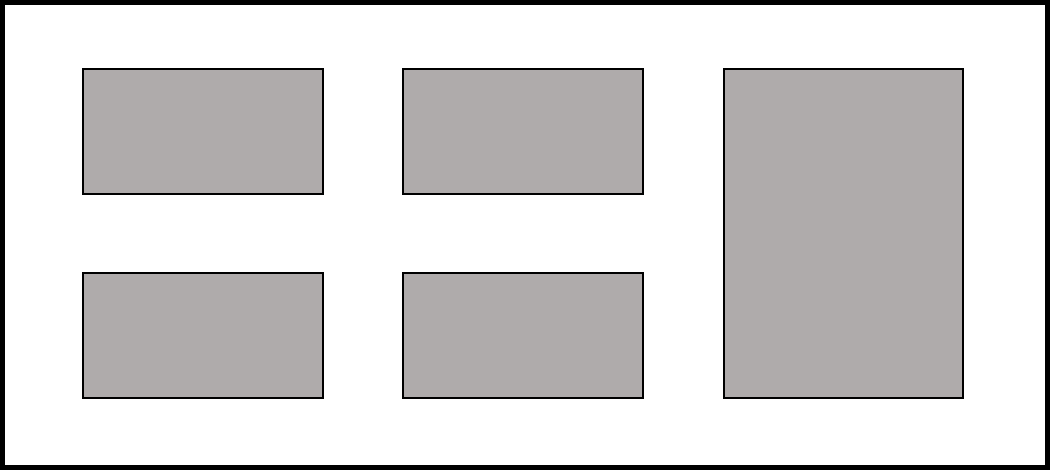
\includegraphics[width=0.7\columnwidth]{Figures/SampleMap2.png}} \\
    \subfigure[Each Vertex contains a corridor between two blocks.]{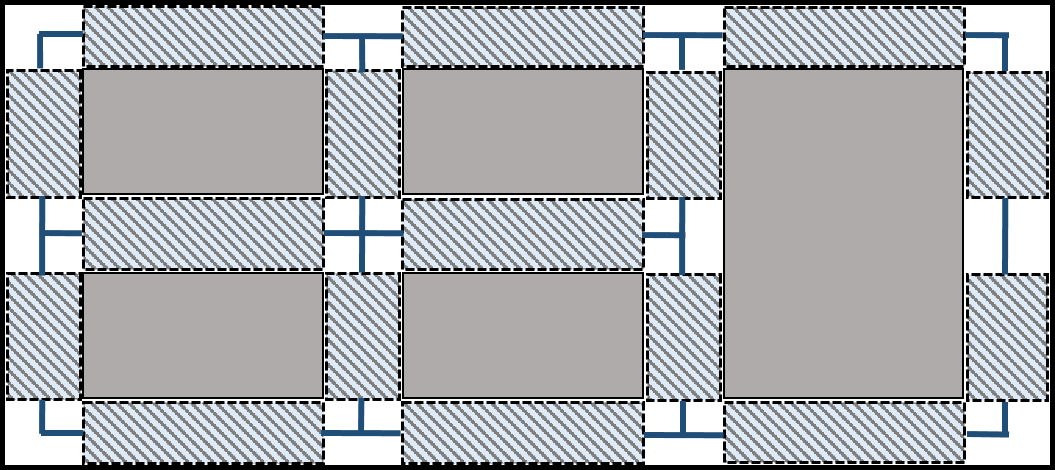
\includegraphics[width=0.7\columnwidth]{Figures/SampleMapWithGraph2.png}} \\
    \subfigure[Corresponding graph.]{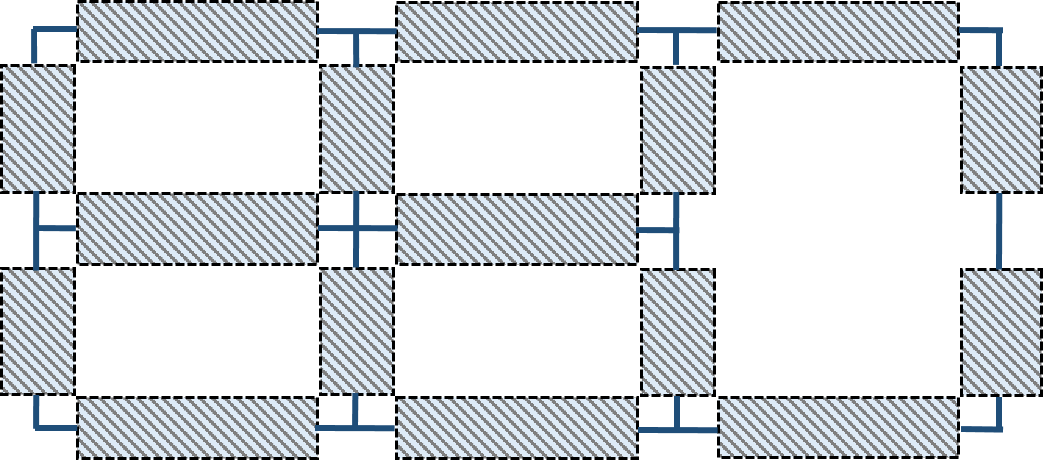
\includegraphics[width=0.7\columnwidth]{Figures/SampleGraph2.png}}    
    \caption{A map with the corresponding graph representation.}
    \label{fig:samplemap}
\end{figure}

%
In Fig.\ref{fig:samplemap} (a) rooms and corridors are shown by gray (obstacles) and white (where robots can move) regions. Vertices area are shaded in (b), and linked by the edges($\mathcal{E}$) placed in the intersections and corners. Finally in (c) the corresponding graph is obtained. The detail of constructing edge set $\mathcal{E}$ is in the continuation.
%%arthur: same thing, isn't this too specific? about lasers and such. maybe the paper should talk about the topological map generically and only specify the sensors in the experimental results, in which we choose a certain type of topological environment to define as nodes and connections. if you agree, I can try to write generically, but more should be placed in the methodology section
%The methodology's basis of work is upon a topological map, represented by a graph, but we propose a specific manner to create such a graph. 

As we are talking about moving robots, it is good to establish a working direction in each region, just as in the real world. For example, there are streets which are only one-way streets and cars can, therefore, only move through them in one direction, while other streets are two-ways and cars can travel in both directions. With this in mind, each region of our topological map will also have either one specific direction of movement or two directions. Then, it is easier if we consider them as separate objects, each with their own connections but also connected between themselves, in the case of two-way regions.

Figure~\ref{fig:numberedGraph} (a) shows one such example. In this case, all of the regions of the graph are bi-directional, thus each one has been separated into two graph nodes. Now, if you want to describe, for example, the connection between the left uppermost region and the right uppermost region, you must specify it using the correct directions of movement between the graph nodes: $1 \rightarrow 3 \rightarrow 5$ is a good way to move there, but $1 \rightarrow 10 \rightarrow 17 \rightarrow 11 \rightarrow 5$ could also be a possible connection. Figure~\ref{fig:numberedGraph} (b) also indicates the two possible paths in blue and green arrows, respectively. 

According to our definition, graph $\mathcal{G}(\mathcal{V},\mathcal{E},\mathcal{C},\mathcal{I})$ contains 4 elements, such that first two sets $\mathcal{V},\mathcal{E}$ have been created so far. In order to create two other set ($\mathcal{C},\mathcal{I}$) proposal explained in Def. \ref{def:commands} is applied.

So that, we define a command $I \in \mathcal {I}$ that describes a required command, $cl \in CL$ to go from one node to another. Therefore, a \textit{''Path"}, \textit{''Commands"} and \textit{''Cost"} between 2 arbitrary nodes ($v_i$ and $v_j$) are described through a list of nodes as following:\\
\\
\begin{figure}[h]
	\centering
	\subfigure[Graph]{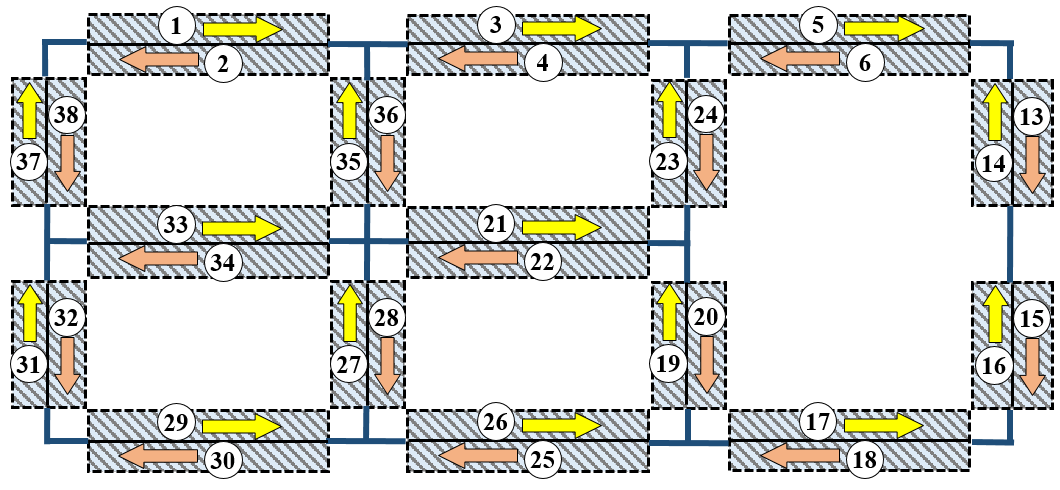
\includegraphics[width=0.8\columnwidth]{Figures/SampleGraphNumbered2.png}}
	\subfigure[Example paths]{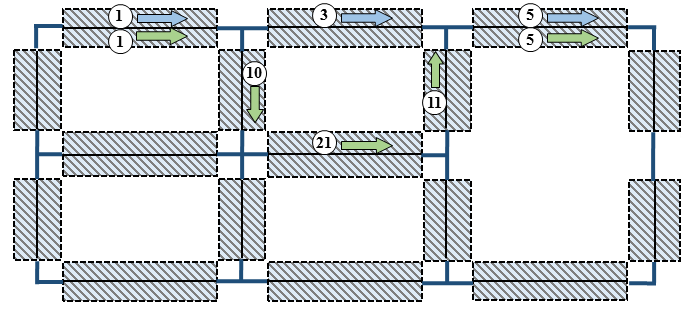
\includegraphics[width=0.8\columnwidth]{Figures/SampleGraphPath.png}} 
	\caption{A graph with numbered nodes and two example paths.}
	\label{fig:numberedGraph}
\end{figure}
%
%
$Path(v_i,v_j)=\{v_i,\cdots,v_k,\cdots,v_j\}, ~~v_i,v_k,,v_j \in \mathcal V$\\
\\
\sloppy $Commands(v_i,v_j)= \{I(v_i,v_{i+1}),\cdots,I(v_k,v_{k+1}),\cdots,I(v_{j-1},v_j)\}\\
=\{cl_{ii},\cdots,cl_{kk},\cdots,cl_{jj}\},$\\
\\
$Cost(v_i,v_j)=\{c(v_i,v_{i+1})+\cdots+c(v_k,v_{k+1})+\cdots+c(v_{j-1},v_j)\}=\sum\limits_{a \in Commands(v_i,v_j)}\tau_a$, 

where $\tau_i \in \mathcal{S}$ is the cost of possible motions.
%
For example the corresponding value for the path shown in Fig. \ref{fig:numberedGraph} (b), with \sloppy $CL=\{Turn\_lef, Turn\_right, Go\_Straight\}$ with $\mathcal S=\{4,4,2\}$ are:

$Path (v_1,v_5)=\{e(v_1,v_3),e(v_3,v_5)\}$,

$Commands(v_1,v_5)=\{I(v_1,v_3),I(v_3,v_5)\}=\{cl_3,cl_3\}$,

$Cost(v_1,v_5)=c(v_1,v_3)+c(v_3,v_5)=\tau_3+\tau_3=4$.
%*********************************
\subsection{Decentralized solution}

We propose a discrete deployment algorithm to lead robots movement towards the center of Voronoi subgraph. The algorithm works in a distributed manner, thus each robot execute one copy of Alg. (\ref{Alg:Depl}).

% algorithm
\begin{algorithm}[H]
  \renewcommand{\algorithmicrequire}{\textbf{Input:}}
    \renewcommand{\algorithmicensure}{\textbf{Output:}}
\caption{$Deployment~Algorithm~for~robot~i$ }
\label{Alg:Depl}
\begin{algorithmic}[1] 
    \REQUIRE $G, r_i, \phi$ The input Graph, initial position of robot $i$ and the density function
%     \ENSURE 
		\WHILE{$(cnt<\beta)$}%cnt<\beta $}
         	\STATE $Broadcast(r_i)$ \COMMENT{ Spread location for neighbors.}
         	\STATE $\mathcal{N}_i \gets Rec\_Neigh\_Pos(G)$ \COMMENT{Receive locational information of robot neighbors.}
           	\STATE $g_i \gets Compute\_Voronoi(G,r_i,\mathcal{N}_i)$ \COMMENT{Compute Voronoi subgraph }
             \STATE $\mathcal{H}_i \gets Compute\_H(r_i,g_i)$
             \FOR{$a \in \mathcal{N}_G(r_i)$} %\COMMENT{Compute $\mathcal{H}$ for each node neighbor.}
             	\STATE $\hat{\mathcal{H}}_i \gets Compute\_H(a,g_i)$
           	\ENDFOR
            \STATE $(\mathcal{H}_i^{min}~, q) \gets MIN(\hat{\mathcal{H}}_i)$ \COMMENT{Find the minimum $\hat{\mathcal{H}}_i$ among the neighbor vertices. }
          		\IF {$\mathcal{\hat{H}}_i^{min} < \mathcal{H}_i$}
                	\STATE $r_i \gets Move\_To(q)$ \COMMENT{Move toward neighbor vertex $q$ and update $r_i$.}
                \ENDIF 
                \STATE $\Delta \mathcal H_i \gets |\mathcal H_i^{t}-\mathcal H_i^{t-1}|$
                \IF{$\Delta H_i < \alpha$} 
                \STATE $cnt=cnt+1$ \COMMENT{Count how many times $\Delta H_i$ is less than $\alpha$ }
                \ENDIF
    	\ENDWHILE
%\STATE $Return\_Failure()$ %\Comment{// Search is unsuccessful.}
\end{algorithmic}
\end{algorithm}

In this algorithm the graph $G$ and $\phi$ are the inputs.At the beginning of the algorithm in line 2, robot broadcasts its locational information to the neighbor robots which are insight of robot's network. This is important since robots do not know how many robots exist in the environment. Also robot $i$ needs its neighbors position, $\mathcal N_i$ in order to compute its Voronoi subgraph (in line 4). After robot computes the deployment function ($\mathcal{H}_i$) upon the established Voronoi subgraph, in lines 6-8 we compute $\hat{\mathcal{H}}$ for all neighbor vertices ($\mathcal{N}_G(r_i)$). 
%
Since robot is able to move to one of its neighbor nodes in each iteration, we estimate the value of $\mathcal{H}$ in the robot's next possible movement to see weather it is worth or not. Thus in line 10 we compare set of $\hat{\mathcal{H}}$, obtained from neighbor vertices, with $\mathcal{H}$ that has computed based on robot current position. 
%

\begin{figure}
\centering
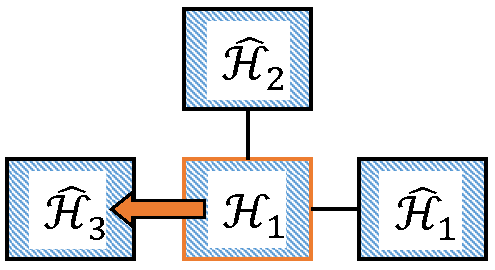
\includegraphics[width=0.35\columnwidth]{Figures/Neighbors.pdf}
\caption{Robot 1 is placed at the center vertex }
\label{fig:neighbors}
\end{figure}

Robot will move to the new vertex if it gets a better (lower) $\mathcal H$. An example is shown in figure \ref{fig:neighbors}, where $\hat{\mathcal{H}}_3<\hat{\mathcal{H}}_2<\hat{\mathcal{H}}_1$ and also $\hat{\mathcal{H}}_3< {\mathcal{H}}_1$. Hence, the vertex labeled $\hat{\mathcal{H}}_3$ is selected as the next node to move. The local search strategy to find the next best movement and minimize the $\mathcal{H}$ is given in Eq. \ref{eq:findmin}.

\begin{equation}
\label{eq:findmin}
q=\arg\min_{a\in \mathcal{N}_G(r_i)} \hat{\mathcal{H}_a},  
\end{equation}
%
It should be noticed that we use the current Voronoi subgraph region to computer $\hat{\mathcal{H}}$ function for neighbor vertices (the input of $Compute\_H$ function is always $g_i$ for all neighbor nodes in line 7). Hence the process of computing the Voronoi subgraph is executes once in each iteration.

The function $Move\_To()$ in line 11 leads the robot to the next vertex ($q$). The controller which used for this purpose is explained in section \ref{sec:robotcontrol}. 

The entire loop in Alg. \ref{Alg:Depl} will repeat the process until the condition $cnt=\beta$ is met. In fact in each iteration the subtraction of current $\mathcal H_i^t$ and previous one ($\mathcal{H}^{t-1}$) determines weather robot has moved or not (in lines 13-16). If robot does not move for specific number of iterations ($\beta$), the algorithm will stop. 
\\
Since the system is distributed, robots' motion affects on others, hence it might happens a robot stops on a vertex for a while, and continue its movement later based on neighbor robots' action. Through this discussion, the algorithm shows that the deployment function $\mathcal{H}$ is decreasing during execution. This property is used in the next section to prove the convergence of robots deployment algorithm.

%*********************************
\subsection{Proof of convergence}

It is important to show that robots will converge to points after being executed for a while. 
In our proposed method in two steps we guarantee this issue:

\begin{itemize}

\item Based on the algorithm \ref{Alg:Depl} we explicitly defined that the execution will continue if the new $\mathcal{H}_i$ is less or equal to the current $\mathcal{H}_i$. Thus we can claim that the value of deployment function make a decreasing sequence. In order to employ this behavior for the proof we first define:

\begin{mydef}[Decreasing sequence]:\\
\textnormal{A sequence $\{x_n\}$ is called decreasing and lower bounded, if:}\\
(1) $~~x_i\leq x_{i-1}~~\forall i \geq 1$\\
(2) $~~\exists B_0 \in \mathbb{R}$ \textnormal{ such } $\forall n ~x_n \geq B_0$\\
\textnormal{
Furthermore, $B=\mathbf{Inf}\{x_n\}_{n=1}^{\infty}$ is called $greatest-lower-bound$ of $\{x_n\}$. Notice that if $\{x_n\}$ is lower bounded, then $B \neq -\infty$
}
\end{mydef}

%----------------------------------
\begin{lemma}[Every lower bounded decreasing sequence converges to the $greatest-lower-bound$ ]
\label{lema1}
\textnormal{By considering:
$B=\mathbf{Inf}\{x_n\}$\\
We want to show that:}\\
%
$\lim\limits_{n \rightarrow \infty}~x_n \rightarrow B$ ~~i.e. \\

$\forall \epsilon>0, ~\exists N_\epsilon ~~$ \textnormal{ such that }$|x_n-B|<\epsilon~~\forall n\geq N_{\epsilon}$

\end{lemma}
%----------------------------------
\begin{proof}:\\
\label{proof1}
The proof is available in \cite{tagkey1997}.
% Since $B+\epsilon$ is not lower bound for $\{x_n\}$, there exist $N_\epsilon$ such that:\\
% \\
% $x_{N_\epsilon} < B+\epsilon$, since $\{x_n\}$ is decreasing:
% \\
% $\forall n\geq N_{\epsilon}$  $x_n<B+ \epsilon$  i.e.
% \\
% $x_n-B<\epsilon, ~\forall n > N_{\epsilon}~ (a)$\\
% \\
% Now, $b-\epsilon$ is a lower bound for $\{x_n\}$, so:\\
% \\
% $ \forall n\geq N,~x_n>B-\epsilon$  i.e. $x_n-B>-{\epsilon} ~(b)$\\
% \\
% Based on $(a)$ and $(b)$ we can conclude:\\

% $\forall n \geq N ~-\epsilon<x_n-B<\epsilon$\\

% $\forall n \geq N ~|x_n-B|<\epsilon$
\end{proof}

Given above explanation, the deployment function $\mathcal{H}$ is decreasing during execution, so that:\\
\\
% $\mathcal{H}: R \times G \rightarrow \mathbb{R}^+$\\
${t}<{t+1} \Rightarrow  \mathcal{H}(t)\geq \mathcal{H}({t+1})$\\
$\forall t \in \mathbb{R} ~~ B\leq \mathcal{H}(t)$, thus: ~~~   $B=\mathbf{Inf} \{\mathcal{H}(t)\}_{t \in \mathbb{R}}$\\

Since the sequence is lower bound to $B$ and decreasing, based on lemma \ref{lema1} we can conclude that $\mathcal{H}$ will converge to a value in $\infty$, consequently robots will stop in some points.
N 
\item In the second step, we refer to the property of Voronoi based motion proposed by Lloyd. For the continues environment proposition (1) and (2) from \cite{Pimenta2008} shows the necessary condition for minimizing the deployment function. The same idea is applicable for the discrete setup and in particular in our proposed method.

If we simply define the objective function for robot $i$ in its Voronoi subgraph $g_i$ as: 
%
\[\mathcal{H}_i=d(g_i,r_i)\cdot \phi(g_i),\]

In our algorithm (lines 6-8), $\mathcal{H}^t_i$ will be computed for all the neighbor set of $r_i$, ($\mathcal{N}_G(r_i)$) based on current Voronoi subgraph ($g_i$). Thus for a neighbor vertex ($q$) which is selected as the next point to go, we already computed $\mathcal{H}_i$.
%
After robot moves to $q$ it will compute $\mathcal{H}^{t+1}$ with a different Voronoi subgraph $\bar{g}_i$, and then we can write:
%
\[d(\bar{g}_i,q)\cdot \phi(\bar{g}_i)<d(g_i,q)\cdot \phi(g_i)\]

It indicates that for a node $q \in \mathcal{G}$, it is always true to say the value of $\mathcal{H}$ in time $t+1$ over subgraph Vornoi $\bar{g}_i$ is lower than the one in time $t$ over $g_i$.

\end{itemize}



%*********************************
\subsection{Implementation of the solution}
\label{sec:robotcontrol}
%in our problem, we would derive the scripts following the shortest way from a node to another one, but here, the nodes are used for your connections and the coverage of area. then, our methodology is simplified to the wall-following based on vector fields.

After the deployment problem has been solved in a certain environment, deployment paths will be generated for each robot involved in the problem. These paths will consist of the nodes through which each robot must move to reach its final position. Then, if a low-level algorithm is used to perform the movements inside each node, a higher-level algorithm can be applied to control the decisions from node to node using the label of the edges. An example will be used to explain this in more detail.

{\color{green}
Reza, can you give me a two robot deployment solution for this sample map? I will try to explain the movements using this
}

Arthur, please try to explain the controller you used to move a robot from a node to another one. You can assume that I give you a \textbf{single command} (not the entire path) i.e. ''Turn left" and then you execute this command based on your wall-following algorithm.

{\color{yellow}
It's because I have to explain an example of a solution by going to my lower level algorithm. As we don't use the shortest path, like I do.
}

%%%%%%%%%%%%%%%%%%%%%%%%%%%%%%%%%%%%%%%%%%%%%%%%%%%%%%%%%%%%%%%%%%%%%%%%%%%%%%%%
\section{Implementation results}
\label{sec:implementation}

The efficiency of the proposed method is investigated in both simulation and real robots experiment.

%*********************************
\subsection{Simulation results}
%
For the simulation we selected a real outdoor map of a neighborhood in New York City from Google Maps (See Fig. \ref{fig:googlemap}). In this map, streets and blocks likely have a symmetric shape, which is important for metropolitan cities in order to facilitate distributing services and urban management i. e. transportation, pipeline, electricity and so on. Furthermore, this block-shape property gives us the ability to run our deployment algorithm without the need of precise localization. Thus, regardless to the scale of the input map, first of all we extract streets from the map in Fig. \ref{fig:googlemap} (b). 

\begin{table}[t]
\centering
\caption{Set of commands and costs in the simulation.}
\label{tbl:commandsets}
\begin{tabular}{cm{1.5cm}cm{1.9cm}cm{1.8cm}}
Command\#  & type  & Cost    \\
\hline\\
1 & Turn\_Left &  1.5 \\
2 & Turn\_Right& 1.5\\
3 & Straight &  1\\
4 & Turn\_Back & 2\\
\hline\\
\end{tabular}
\end{table}

%
While the direction of the streets is available in Google map, a directed graph $G$ constructed based on this map (the method was explained in section \ref{sec:topologymap}). The command set $\mathcal{I}$ and its corresponding cost $\mathcal{C}$ that used in this simulation is shown in table \ref{tbl:commandsets}.

% But in the final topological representation moreover than what common method do to create the graph and costing the edges, we create a label set $\mathcal{I}$ that indicates the action to move from a vertex to its neighbor. 
%
After having $G$, we distribute 6 robots randomly over the environment. Robots are equipped with laser sensor to move through the streets by following the walls. 
%
In real example scenario, assume that 6 police cars must cover this neighborhood to avoid evading a criminal car. After applying algorithm \ref{Alg:Depl}, robots' final location, assigned region and the traversed path are depicted in Fig. \ref{fig:googledeployed} (a) with different color. The video is available in following link, \href{https://youtu.be/yAyio1--viA}{https://youtu.be/yAyio1--viA}.

\begin{figure}[h]
	\centering	
	\subfigure[Sattelite view.]{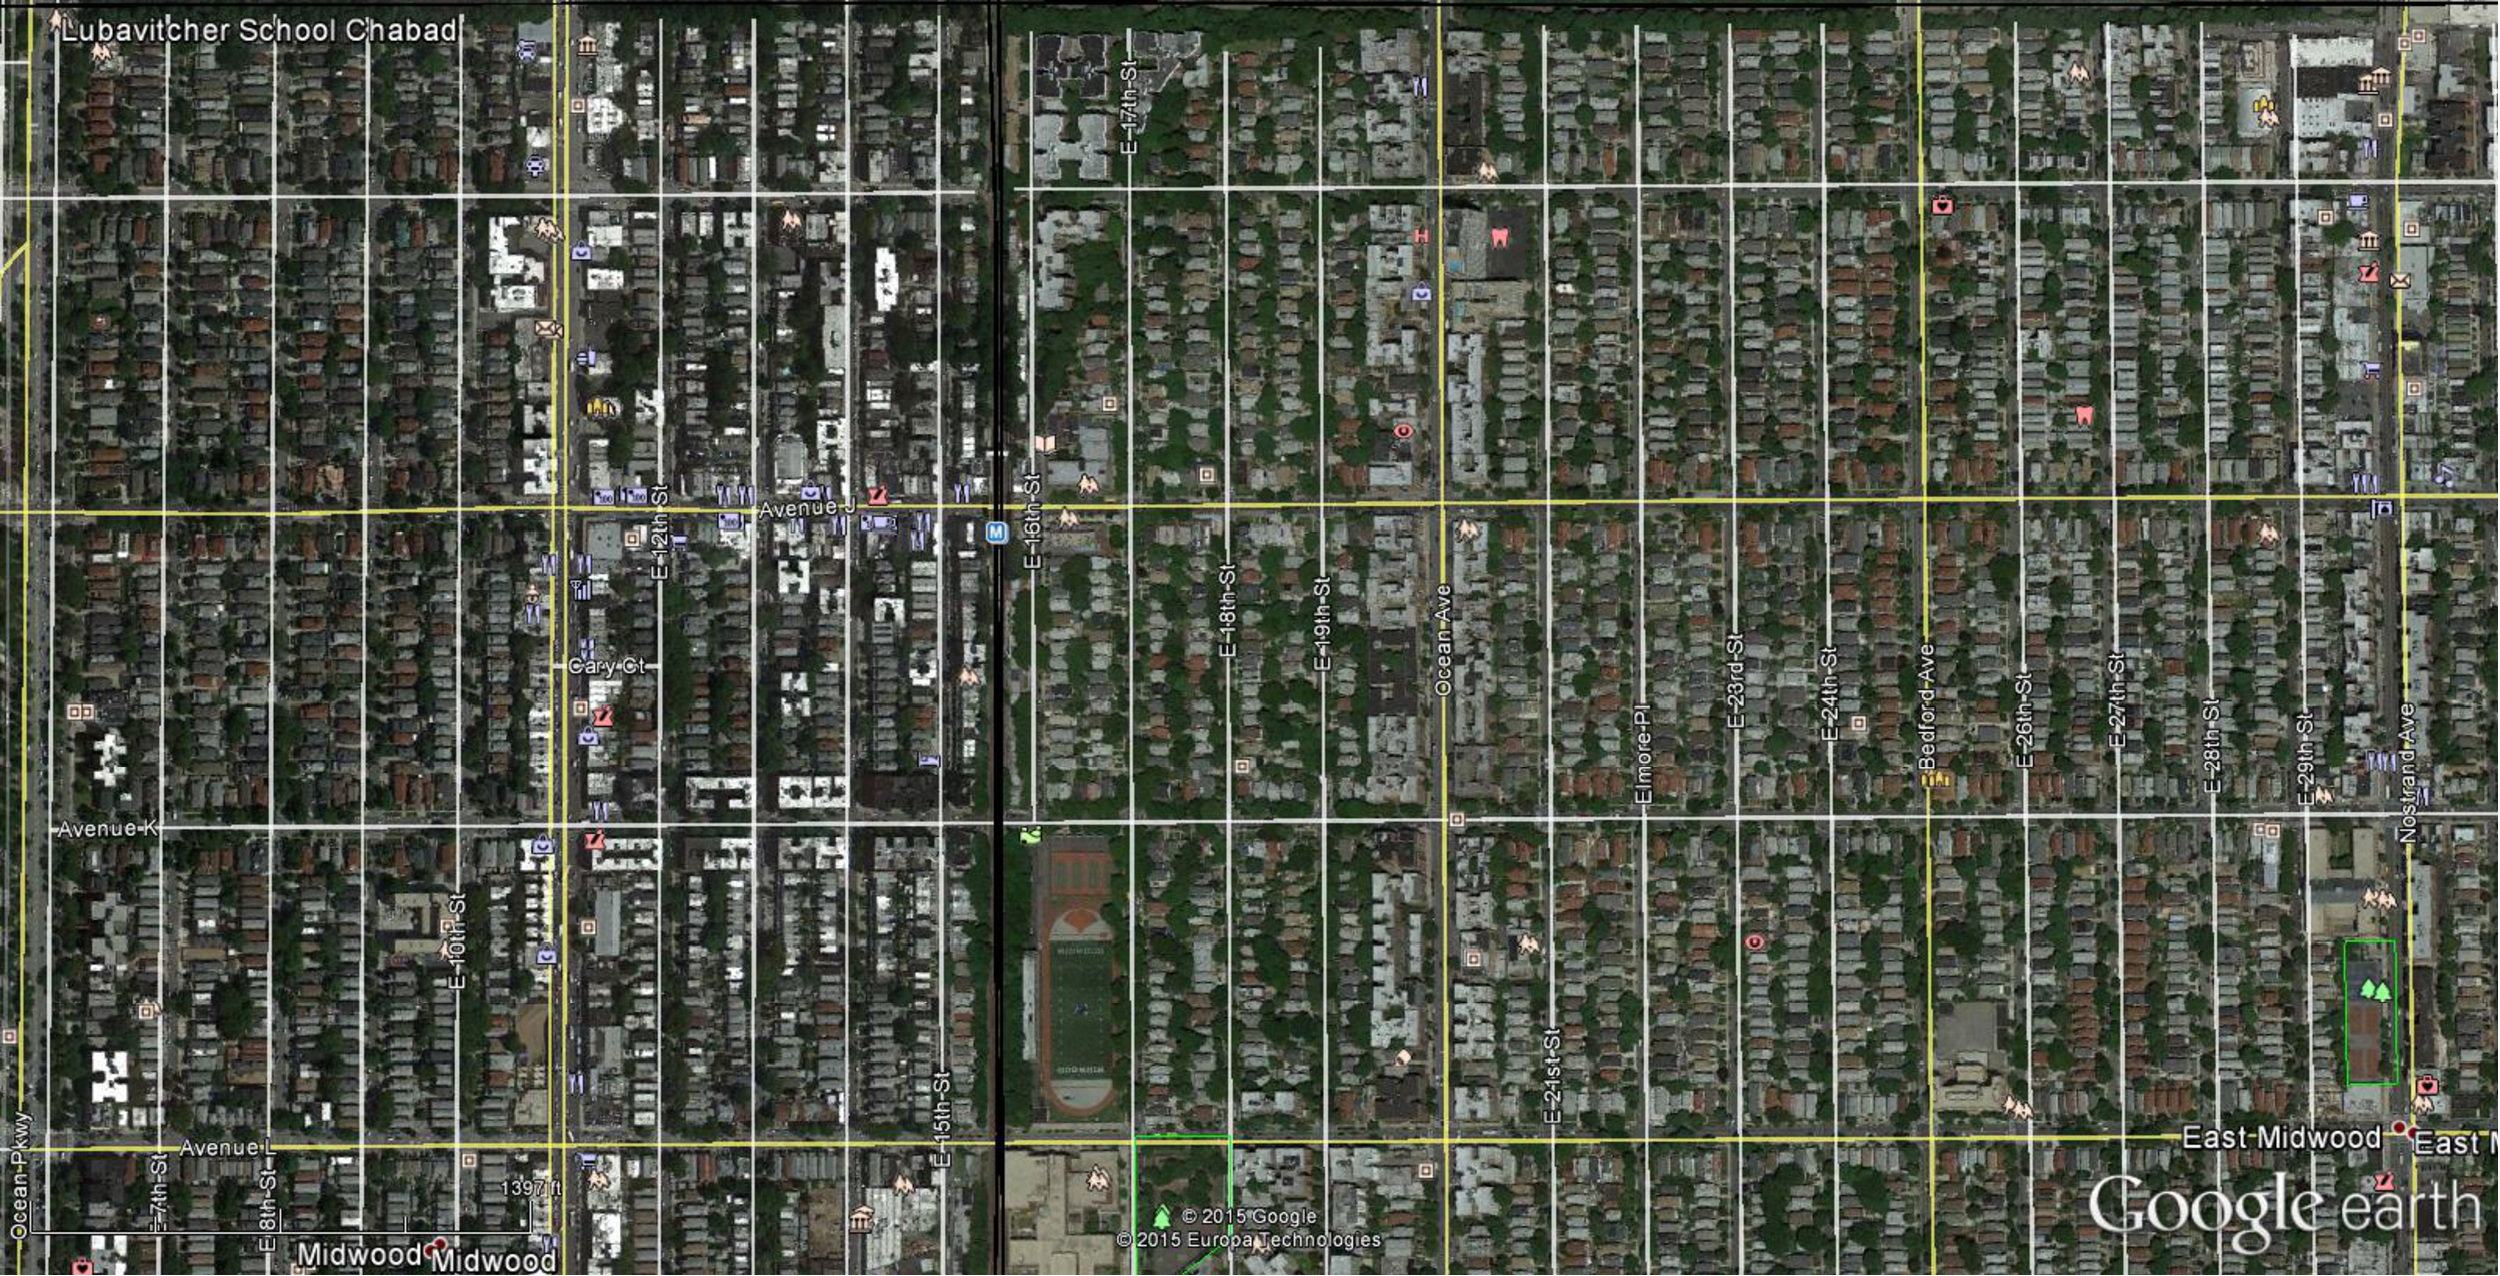
\includegraphics[width=0.8\columnwidth]{Figures/map4lables.pdf}}
	\subfigure[Direction of streets.]{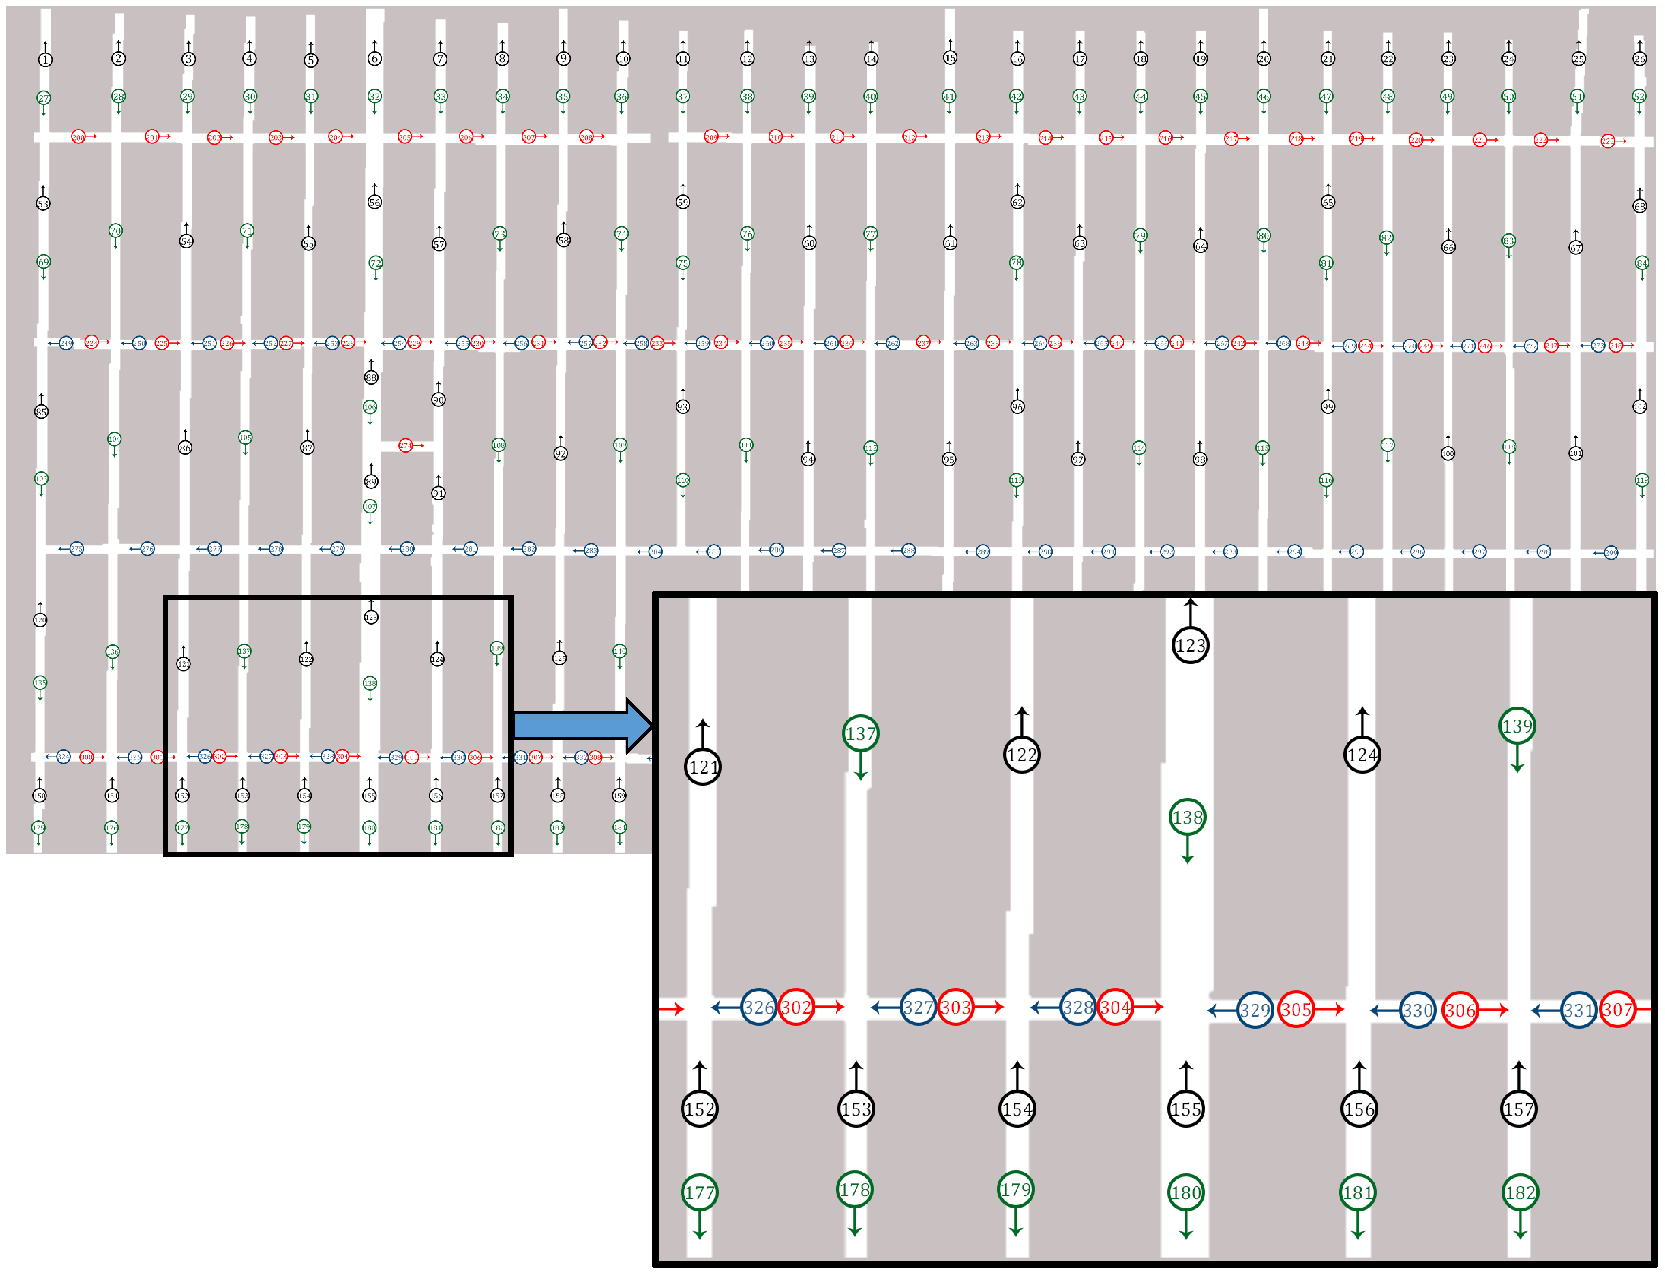
\includegraphics[width=0.8\columnwidth]{Figures/GoogleMapZoom.pdf}}
	\caption{A map grabbed from Google map.}
	\label{fig:googlemap}
\end{figure}
%

In order to investigate the affordance of our on-line method, we performed an off-line $p$-median solution (\cite{Daskin2015}) which is applicable for similar purpose on graph. In this problem, by considering a graph with $n \times m$ vertices, the objective is to assign $n$ facilities between $m$ customers. One of the methods to solve this NP-hard problem is solving Mixed Integer Linear Programming (MILP) which yields the global solution (\cite{Edson2005}).

In this simulation, after applying a solver on the MILP model which takes hours for the graph with $\mathcal{V}=347$, Fig. \ref{fig:googledeployed} (b) contains the result. Moreover, the value of $\mathcal{H}$ function of both methods are shown in table \ref{tbl:comparison}.

\begin{table}[t]
\centering
\caption{Comparison of $\mathcal{H}$ in different methods. }
\label{tbl:comparison}
\begin{tabular}{m{3cm}m{1.2cm}}
Methodology    & Cost($*10^5$)    \\
 \hline\\
 Global Solution   &  1.12686  \\
Proposed algorithm & 1.18786  \\
\hline\\
\end{tabular}
\end{table}

\begin{figure}[h]
	\centering	
% 	\subfigure[Proposed algorithm.]{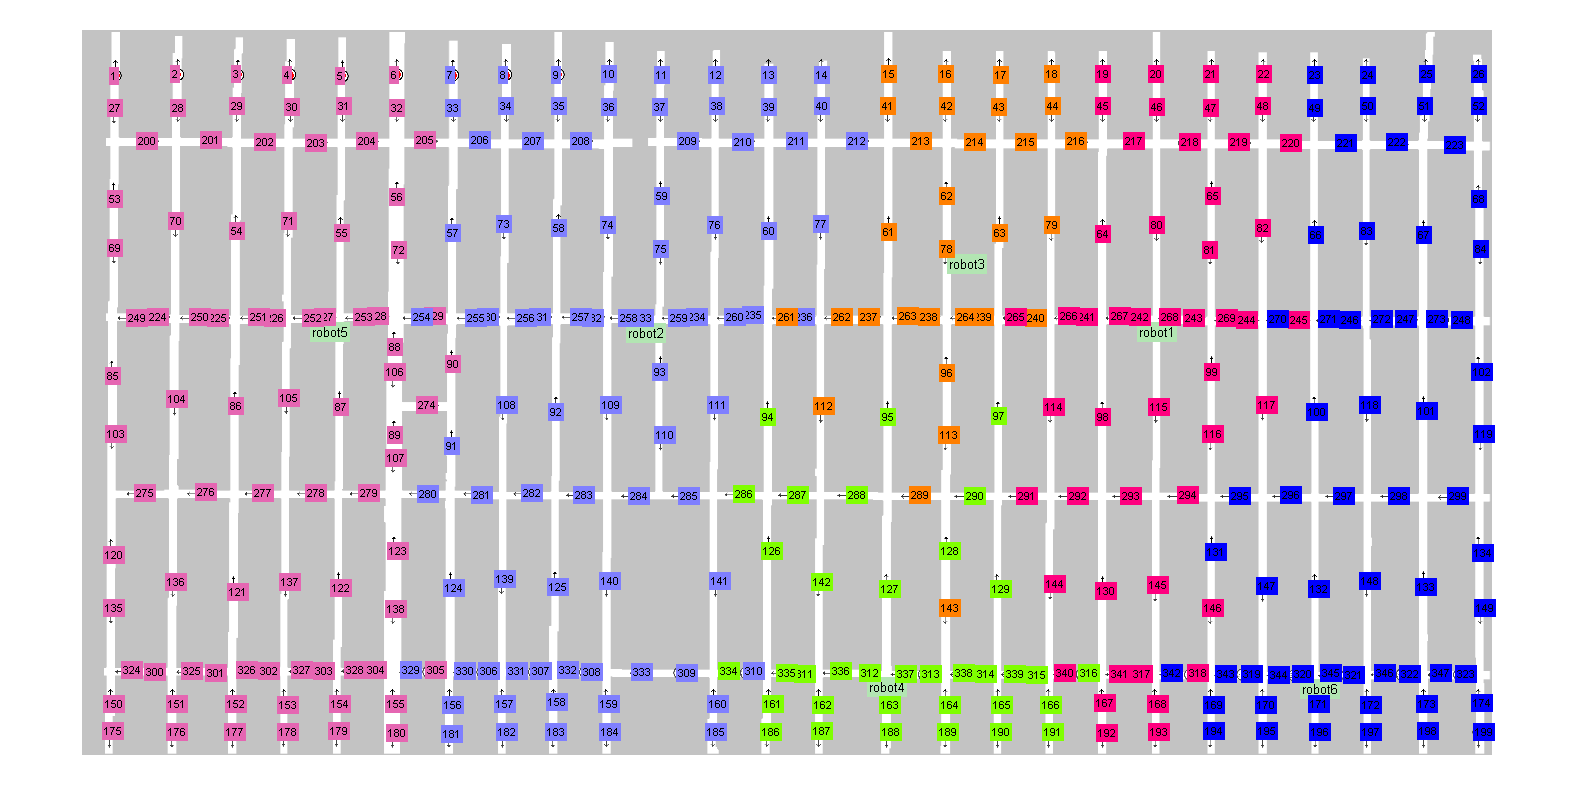
\includegraphics[width=0.89\columnwidth]{Figures/googlemapVD.png}}
     \subfigure[Voronoi regions and the traversed trajectory by robots.]{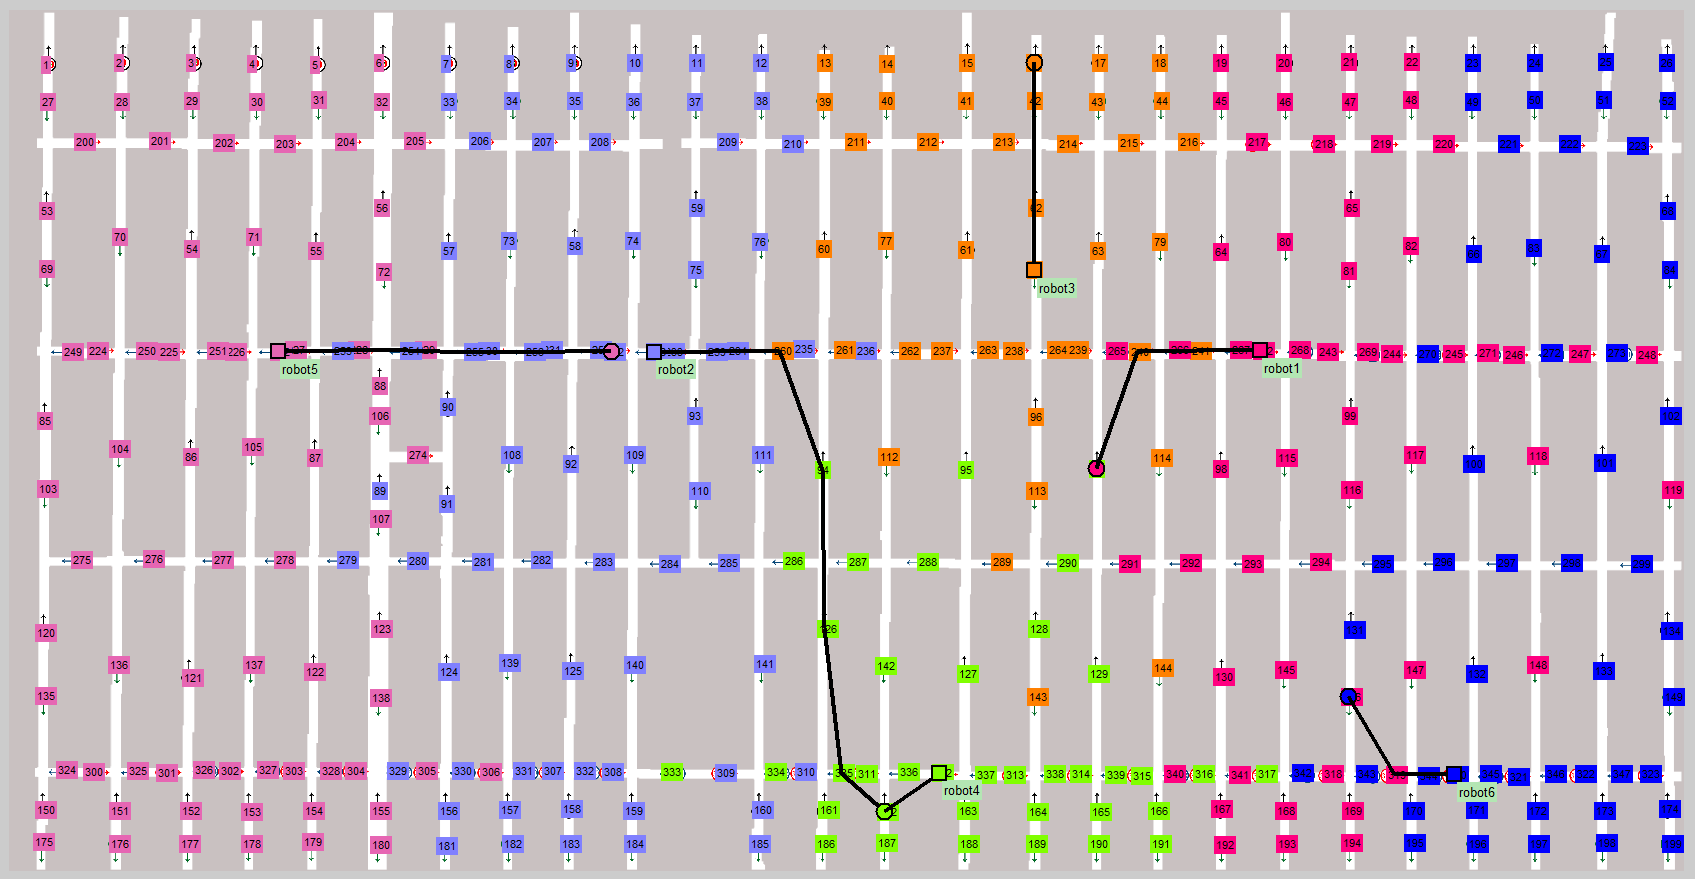
\includegraphics[width=0.8\columnwidth]{Figures/googlemapVDTraj.png}}
    	\subfigure[Global solution.]{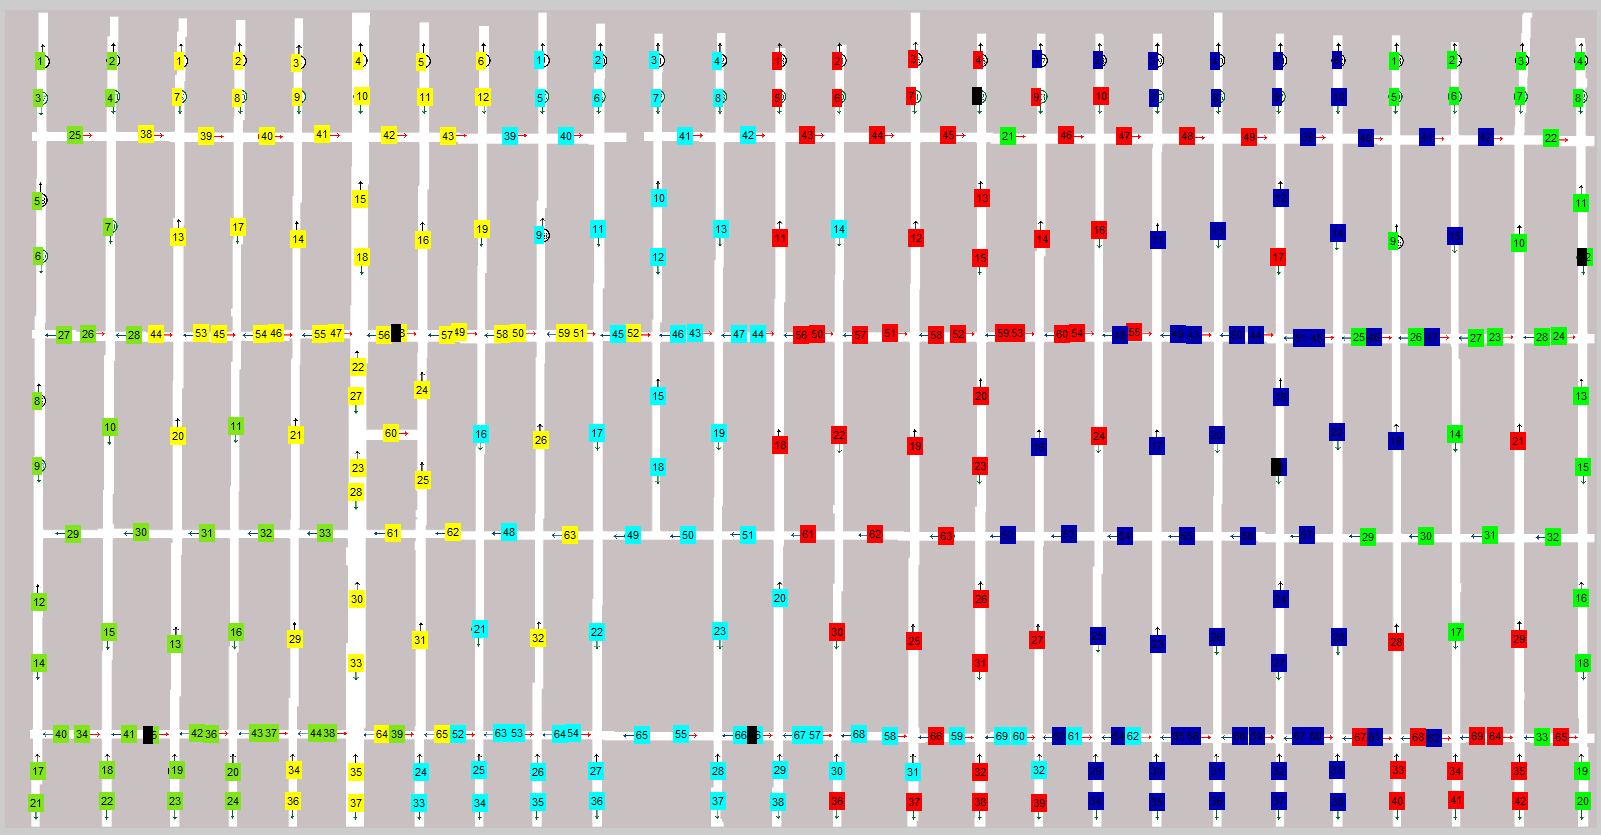
\includegraphics[width=0.8\columnwidth]{Figures/googlemapGlobalVD.png}}
	\caption{Partitioning the map between robots for deployment purpose.}
	\label{fig:googledeployed}
\end{figure}

\begin{figure}
\centering
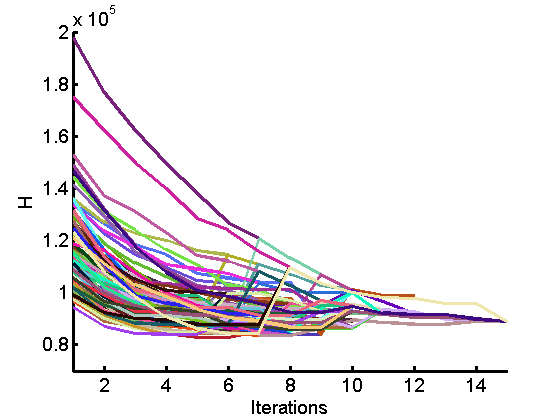
\includegraphics[width=0.8 \columnwidth]{Figures/googlemapH100Times.png}
\caption{Result of running 100 times.}
\label{fig:100sim}
\end{figure}

In our algorithm function $\mathcal{H}$ evolves over time, the result of 100 times running the proposed method on Google map scenario is illustrated in Fig. \ref{fig:100sim}. In each simulation robots are redistributed randomly in the initial positions, and after executing maximum 14 times, robots converged about final position. It is important to remark that in order to move in such a big map, in our method only few human-like commands are enough to get from a point (or street) to another.

%you could say here that the deployment problem is then considered as covering the most even number of streets as regions, or of nodes, depending on how you are doing it. then, talk about the offline planning and that the robots, representing cars, would follow the best solution like that. I don't know if is is good to mention that our moving algorithm here is the same one of the vector fields that would be explained in the next section. if not, then the simulation is also more generic, just showing their movements around the map.

%*********************************
\subsection{Real robot experiments}
%with 3 real robots

%remembering that the algorithm needs to know the initial position of the robots, but now the robots only follow orders.

After validating the performance of proposed method through the simulation, experiments were performed to testify its applicability in the real world. Thus, three robots were chosen to be used in this experiment.

Two of the robots are based on the same mobile base, that of a Pioneer P3-AT \footnote{http:\/\/www.mobilerobots.com\/ResearchRobots\/P3AT.aspx}. They are non-holonomic robots with four wheels, used in conjunction with a laser range sensor and odometric sensors. The first Pioneer, which we will call Robot 1, has indoors wheels and a SICK LMS100 laser\footnote{http:\/\/www.sick.com} range sensor, while the second robot, to be called Robot 2, has outdoor wheels and a SICK LMS291 laser range sensor. 
% The LMS100 is an Ethernet-based laser, receiving laser information of up to 20 meters of distance, 50 times per second. Meanwhile, the LMS291 is an RS422-based laser, receiving laser information of up to 8 meters of distance, 9 times per second.

The third robot, Robot 3, has a small iRobot Create mobile base \footnote{http:\/\/store.irobot.com}, with three wheels. It also has odometric sensors and a Hokuyo URG \footnote{https:\/\/www.hokuyo-aut.jp} laser range sensor. 
% This laser sensor gives, 10 times per second, laser data of up to 5.6 meters of distance through a USB connection.

The experiments were done in the School of Engineering building of the Federal University of Minas Gerais. It is a symmetrical building, and is composed of many corridors and intersections (See Fig \ref{fig:depmap} (a)). To build the correspondent graph, the corridors were separated into the nodes of the graph, one node for each direction of movement, while the edges consist in the intersections. Each edge received a label with the direction to which the robot had to turn to reach the new corridor in an intersection. 

\begin{figure}
\centering
\subfigure[Map is captured from Google map.]{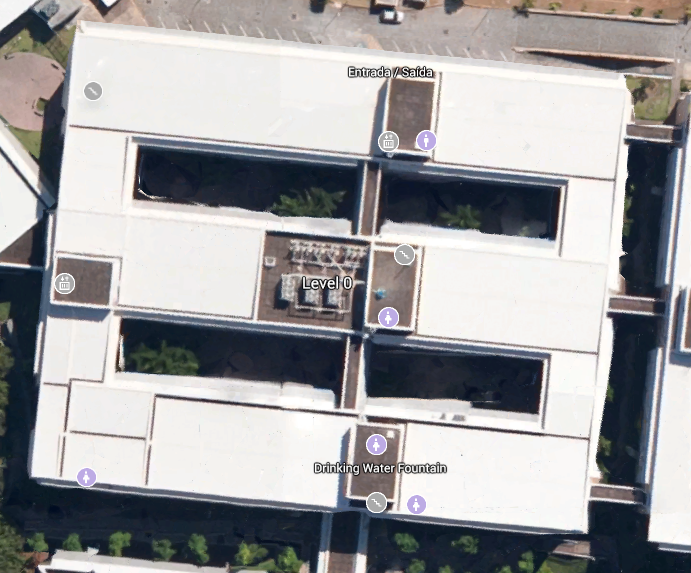
\includegraphics[width=0.5 \columnwidth]{Figures/ElecEngDep.png}}
\subfigure[Representing the input map as a graph.]{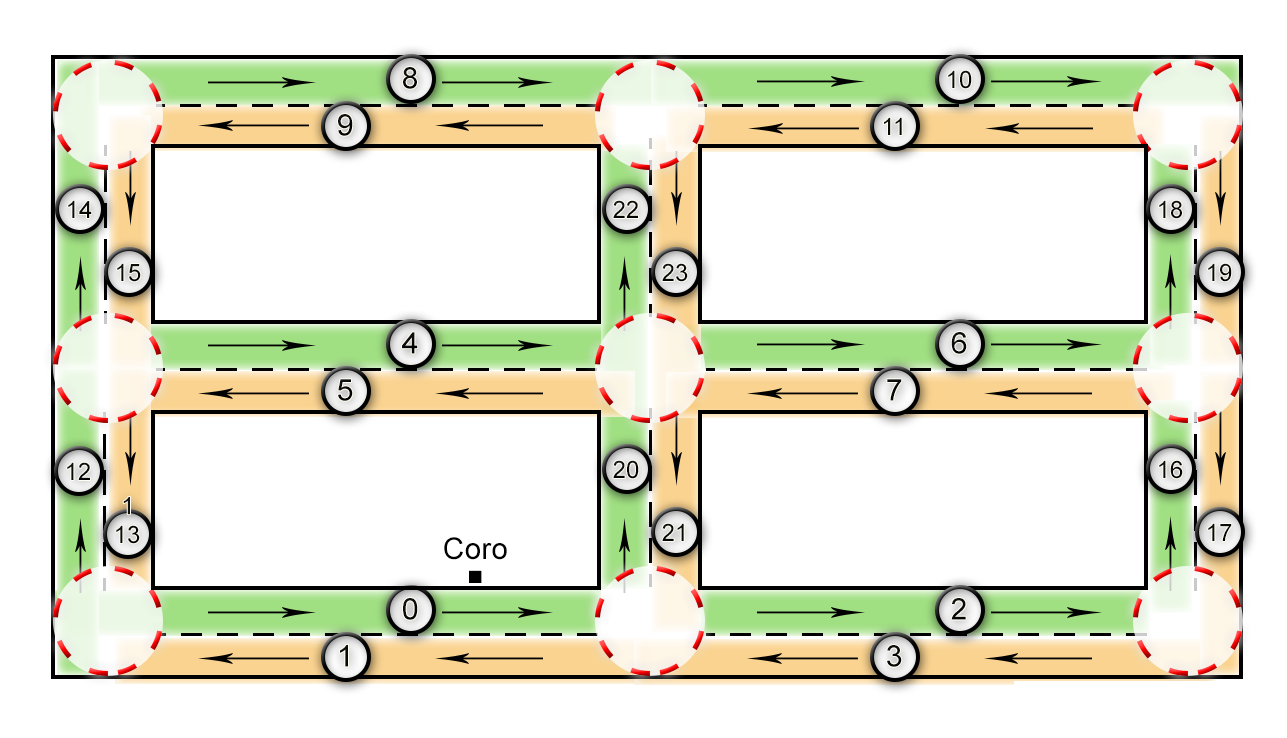
\includegraphics[width=0.75 \columnwidth]{Figures/general_map.png}}
\caption{The map used in real robot experiment.}
\label{fig:depmap}
\end{figure}

\begin{figure}
\centering
\subfigure[Initial position with corresponding Voronoi subgraph with different color]{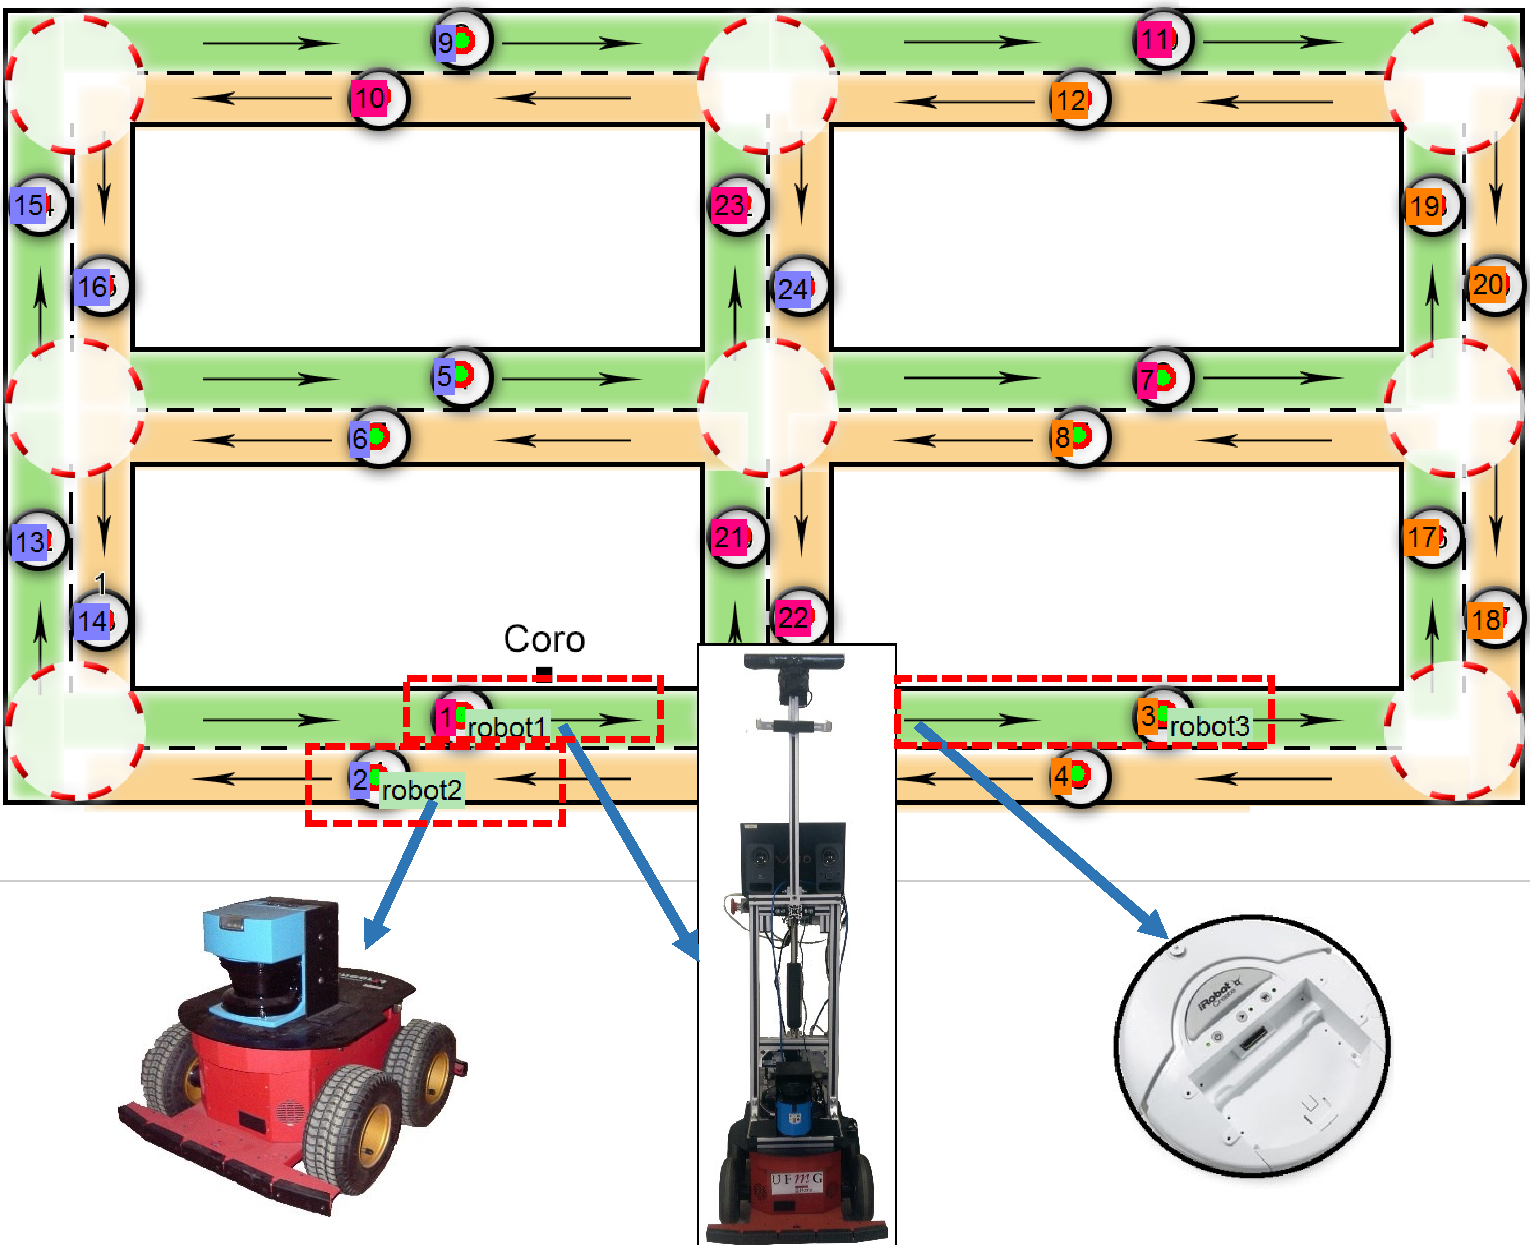
\includegraphics[width=0.7 \columnwidth]{Figures/robots.pdf}}
\subfigure[Final Deployment]{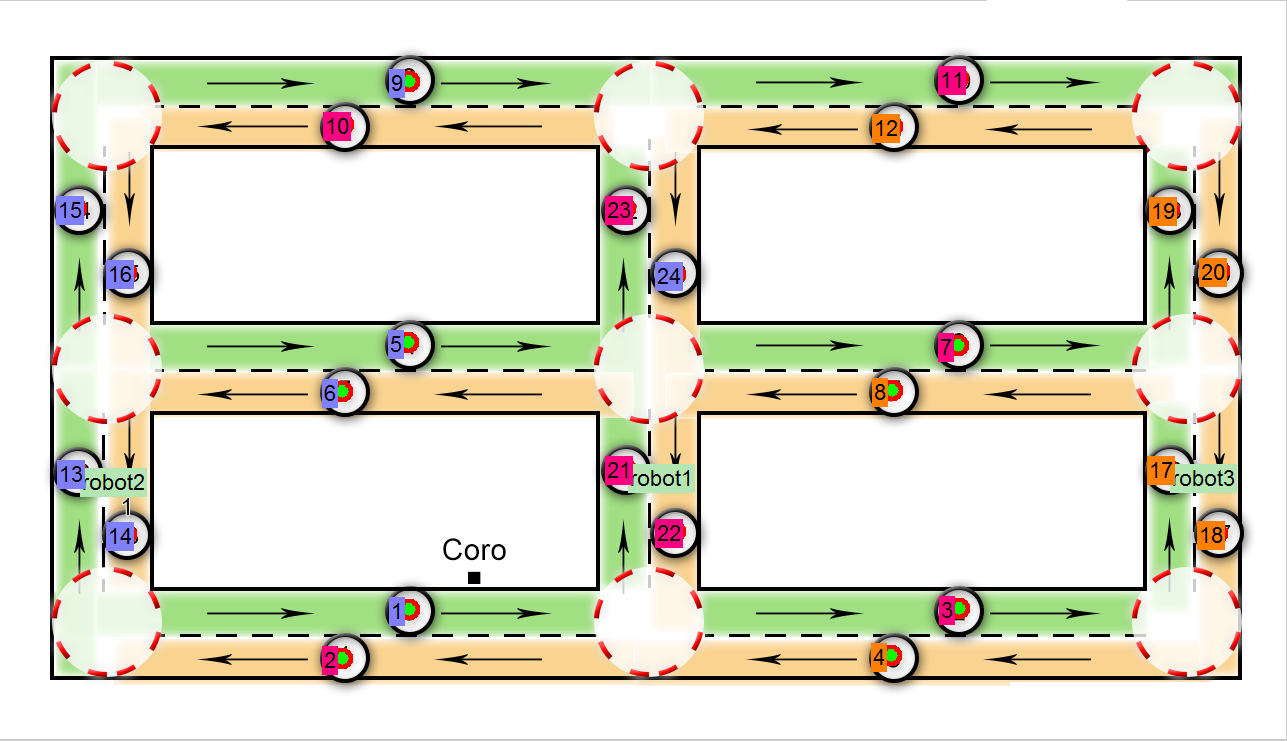
\includegraphics[width=0.73 \columnwidth]{Figures/DepFinalDep2.png}}
\caption{Deployment of 3 robots in a real scenario.}
\label{fig:depmapDeploy}
\end{figure}


Figure \ref{fig:depmap} (b) shows the topological map of the environment, with 24 nodes. 

The initial vertices, and the final deployment location are depicted in figure \ref{fig:depmapDeploy}. So that, robots 1,2 and 3 started from vertices 1, 2 and Robot 3 (See (a)), and ended on vertices 21, 13 and 17 (see (b)), respectively. In the Entire execution each robot runs a single command (See table \ref{tbl:commands}). The complete video of this experiment can be found in \href{https://youtu.be/SETuu-FbI0I}{https://youtu.be/SETuu-FbI0I}.

\begin{table}[t]
\centering
\caption{Commands applied on robots in the real experiment. }
\label{tbl:commands}
\begin{tabular}{cm{2cm}m{1.2cm}}
Robot\#    & command    \\
\hline\\
1   & Turn\_Left   \\
2 &  Turn\_Right \\
3 & Turn\_Left \\
\hline\\
\end{tabular}
\end{table}

{\color{red}
First, the deployment problem was solved offline, and then the solution for each robot was loaded in each one as a script of which movements they had to perform to reach their final positions. 
}

A wall-following algorithm was implemented for each robot as the low-level algorithm to move inside the nodes as we explained in section \ref{sec:robotcontrol}. The 
{\color{green}would we explain the basics of the wall-following here?}

%%%%%%%%%%%%%%%%%%%%%%%%%%%%%%%%%%%%%%%%%%%%%%%%%%%%%%%%%%%%%%%%%%%%%%%%%%%%%%%%
\section{CONCLUSIONS}
\label{sec:conclusion}

In this paper, we proposed a distributed multi-robot deployment method based on a topological representation of environment. A practical technique was applied in order to simplify a multi-dimensional map into a single one. This technique can be applicable not only on very large maps, but also works fine in block-shape environment by decreasing the dimension and computation cost relatively.
%
Once the topological model of the input map is obtained, robots use a wall following control to move in the filed, hence no precise localization is needed. This is done by using a natural scheme of navigation, such that robots move to a location by following a sequence of human like commands. 
%
In comparison with different techniques introduced in state of the art for deployment problem, our method has a good affordance in the real application because of the low computation and no need of precise localization. These remarkable properties make our method fast enough to be executed in the real world scenarios. This issue can also be considered as a shortage in such application that having an accurate localization system is necessary.
%
For the future work, we would like to perform real experiments in multi-floor map. Also combining aerial and ground based robots in the deployment mission is our interest. 

%%%%%%%%%%%%%%%%%%%%%%%%%%%%%%%%%%%%%%%%%%%%%%%%%%%%%%%%%%%%%%%%%%
\section*{ACKNOWLEDGMENT}

We are acknowledging that this work was supported by Brazilian agencies, CAPES, CNPq, UFMG.

%%%%%%%%%%%%%%%%%%%%%%%%%%%%%%%%%%%%%%%%%%%%%%%%%%%%%%%%%%%%%%%%%%%%%%%%%%%%%%%
\bibliographystyle{spbasic}
\bibliography{MyReferences} 

\end{document}

